%        File: defense.tex
%     Created: Sun May 5 10:00 PM 2013 C
%


%\documentclass[11pt,handout]{beamer}
\documentclass[9pt]{beamer}
\usetheme[white]{Wisconsin}
%\title[short title]{long title}
\title[Integrated Used Fuel Disposition and Generic Repository Modeling ]{ An Integrated Used Fuel Disposition and Generic Repository Model for Fuel Cycle Analysis }
%\subtitle[short subtitle]{long subtitle}
\subtitle[PhD Oral Examination]{}
%\author[short name]{long name}
\author[Kathryn D. Huff]{Kathryn D. Huff \\ PhD Candidate}
%\date[short date]{long date}
\date[5.17.2013]{May 17, 2013}
%\institution[short name]{long name}
\institute[UW-Madison]{University of Wisconsin-Madison}

%\usepackage{bbding}
\usepackage{amsfonts}
\usepackage{amsmath}
\usepackage{xspace}
\usepackage{graphicx}
\usepackage{subfigure}
\usepackage{booktabs} % nice rules for tables
\usepackage{microtype} % if using PDF
\usepackage{bigints}
\newcommand{\units}[1] {\:\text{#1}}%
\newcommand{\SN}{S$_N$}%{S$_\text{N}$}%{$S_N$}%
\DeclareMathOperator{\erf}{erf}
\newcommand{\Cyder}{\textsc{Cyder}\xspace}
%I need some complimentary error funcitons... 
\DeclareMathOperator{\erfc}{erfc}
%page numbers
\setbeamertemplate{footline}[page number]
\setbeamertemplate{caption}[numbered]
%Those icons in the references are terrible looking
\setbeamertemplate{bibliography item}[text]
\begin{document}
%%%%%%%%%%%%%%%%%%%%%%%%%%%%%%%%%%%%%%%%%%%%%%%%%%%%%%%%%%%%%
%% From uw-beamer Here's a handy bit of code to place at 
%% the beginning of your presentation (after \begin{document}):
\newcommand*{\alphabet}{ABCDEFGHIJKLMNOPQRSTUVWXYZabcdefghijklmnopqrstuvwxyz}
\newlength{\highlightheight}
\newlength{\highlightdepth}
\newlength{\highlightmargin}
\setlength{\highlightmargin}{2pt}
\settoheight{\highlightheight}{\alphabet}
\settodepth{\highlightdepth}{\alphabet}
\addtolength{\highlightheight}{\highlightmargin}
\addtolength{\highlightdepth}{\highlightmargin}
\addtolength{\highlightheight}{\highlightdepth}
\newcommand*{\Highlight}{\rlap{\textcolor{HighlightBackground}{\rule[-\highlightdepth]{\linewidth}{\highlightheight}}}}
%%%%%%%%%%%%%%%%%%%%%%%%%%%%%%%%%%%%%%%%%%%%%%%%%%%%%%%%%%%%%
%%--------------------------------%%
\frame{
  \titlepage
}

\section{Motivation}
%%--------------------------------%%
\begin{frame}
  \frametitle{Outline}
  \tableofcontents[currentsection]
\end{frame}

\subsection{Fuel Cycle Simulator Capabilities}


% They just report mass flows
% or are proprietary and super long running

\begin{frame}[ctb!]
  \frametitle{Need For an Integrated Repository Model}

  %        File: systools_tab.tex
%     Created: Mon Aug 29 09:00 AM 2011 C
% Last Change: Mon Aug 29 09:00 AM 2011 C
%
\begin{table}
  \centering
  \footnotesize{
  \begin{tabular}{|l|l|c|c|c|}
    \multicolumn{5}{c}{\textbf{Repository Capabilities within Systems Analysis Tools}}\\
    \hline
    Tool & Institution & Fuel Disposition & Radionuclide Transport & Heat Transport  \\
    \hline
    NUWASTE\cite{abkowitz_nuclear_2010} & NWTRB & yes & no & no \\
    VISION \cite{yacout_vision_2006} & INL   & yes & no & YMR only \\
    DANESS \cite{van_den_durpel_daness:_2006} & ANL   & no & no & no \\
    COSI   \cite{boucher_international_2010} & CEA   & yes & no & yes \\
    NFCSim \cite{schneider_nfcsim_2004} & LANL  & no & no & no \\
    CAFCA  \cite{guerin_benchmark_2009} & MIT   & no & no & no \\
    ORION  \cite{guerin_benchmark_2009} & BNL   & no & no & no \\
    TSM    \cite{turner_discrete_2010} & OCRWM & yes & no & YMR only \\
    \hline
  \end{tabular}
  \caption[System Tools]{System tools are lacking in radionuclide transport and  
  heat transport calculations in generic geolgies.}
  \label{tab:systools}
  }
\end{table}




\end{frame}

\begin{frame}[ctb!]
\frametitle{Contributions from This Work}

This work has provided a platform capable of bridging the gap between fuel cycle 
simulation and repository performance analysis.

  \begin{itemize}
  \item Conducted thermal transport sensitivity analyses. \cite{huff_numerical_2012, huff_benchmarking_2012}
  \item Conducted contaminant transport sensitivity analyses. \cite{huff_key_2012}
  \item \Cyder acheived integration with a fuel cycle simulator.
  \item Abstracted physical models of thermal and contaminant transport. \cite{huff_hydrologic_2013}
  \item Demonstrated dominant physics of those models in \Cyder, integrated 
  with \Cyclus. \cite{huff_dyanmic_2013, huff_cyclus_2013}
  \item Published source code, documentation, and testing to facilitate 
  extension by external developers. \cite{huff_cyder_2013}
  \end{itemize}
\end{frame}

\subsection{Future Fuel Cycle Options}
\begin{frame}[ctb!]
  \frametitle{Top Level Fuel Cycle Simulators}
  % most only report mass flows.
  \begin{figure}[htbp!]
    \begin{center}
      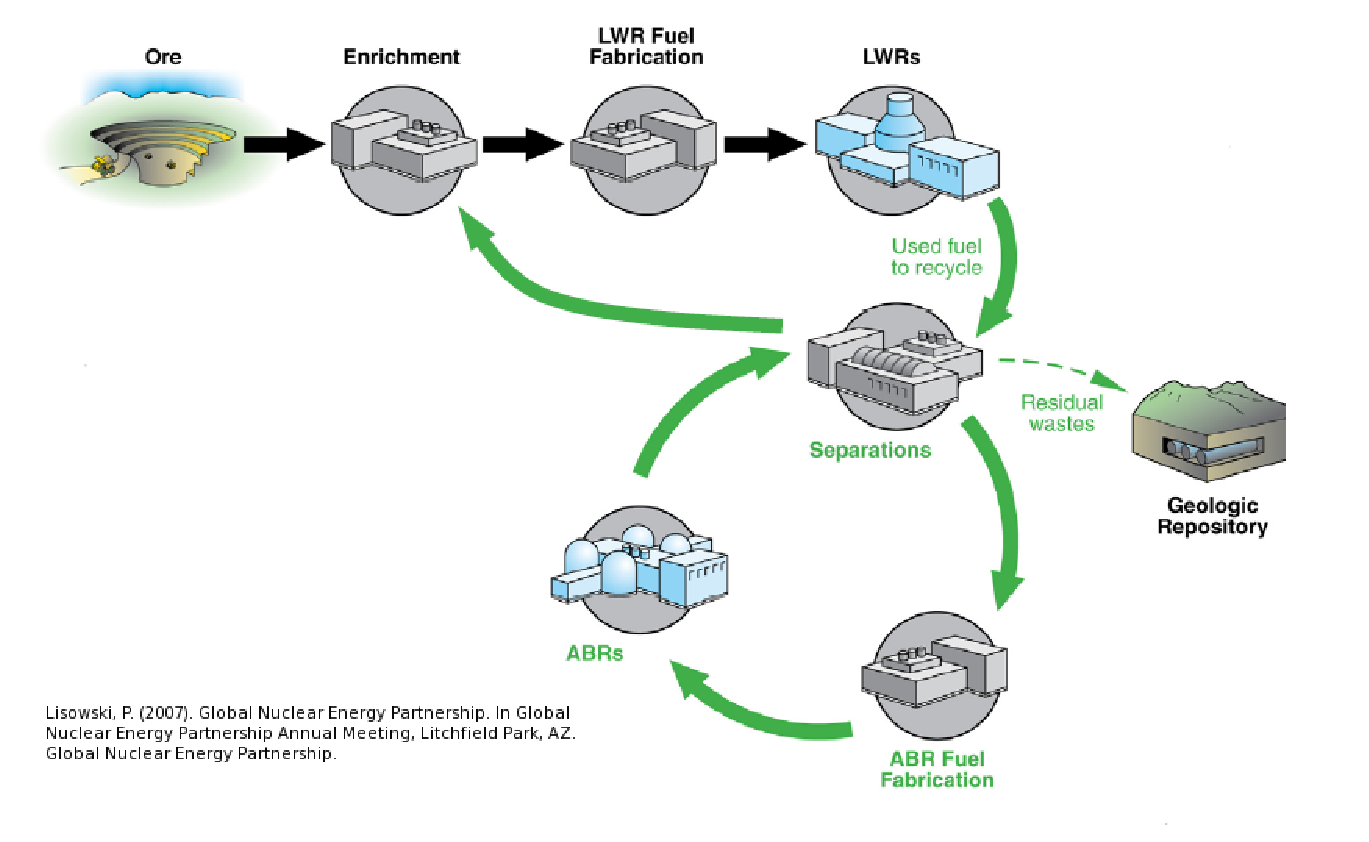
\includegraphics[height=4cm]{./images/simulations.eps}
    \end{center}
    \caption{Top level simulators are intended to model the collective 
    behavior of various fuel cycle decisions and 
    strategies \cite{lisowski_global_2007}.}
    \label{fig:simulation}
  \end{figure}
\end{frame}

\begin{frame}[ctb!]
  \frametitle{Future Fuel Cycle Options}
    \input{fco_tab}
\end{frame}

\subsection{Geologic Disposal Concept Options}


%%----------------------------------------%%
\begin{frame}[ctb!]
  \frametitle{Repository Components}
\footnotesize{
  \input{skb_fig}
}
\end{frame}

\begin{frame}
  \frametitle{Repository Layouts}

  \begin{minipage}{0.49\textwidth}
    \begin{figure}[h!]
      \includegraphics[width=0.75\textwidth]{./images/boreholes.eps}
    \end{figure}
    \begin{figure}[h!]
      \includegraphics[width=0.75\textwidth]{./images/vertical.eps}
    \end{figure}
  \end{minipage}
  \hspace{0.01cm}
  \begin{minipage}{0.49\textwidth}
    \begin{figure}[h!]
      \includegraphics[width=0.8\textwidth]{./images/horizontal.eps}
    \end{figure}
    \begin{figure}[h!]
      \includegraphics[width=0.8\textwidth]{./images/alcoves.eps}
    \end{figure}
  \end{minipage}

\end{frame}



\begin{frame}[ctb!]
  \frametitle{Disposal Geology Options Considered}
   \begin{minipage}{0.44\textwidth}
     \begin{figure}[h!]
         \includegraphics[width=0.7\textwidth]{./images/saltNewScientist.eps}
         \caption{U.S. Salt Deposits, ref. \cite{newscientist_where_2011}.}
     \end{figure}
     \begin{figure}[h!]
         \includegraphics[width=0.7\textwidth]{./images/clayGonzales.eps}
         \caption{U.S. Clay Deposits, ref. \cite{gonzales_shales_1985}.}
     \end{figure}
   \end{minipage}
   \begin{minipage}{0.44\textwidth}
     \begin{figure}[h!]
         \includegraphics[width=0.7\textwidth]{./images/boreholeNewScientist.eps}
         \caption{U.S. Crystalline Basement, ref.  \cite{newscientist_where_2011}.}
     \end{figure}
     \begin{figure}[h!]
         \includegraphics[width=0.7\textwidth]{./images/graniteBush.eps}
         \caption{U.S. Granite Beds, ref. \cite{bush_economic_1976}.}
     \end{figure}
   \end{minipage}
\end{frame}


\section{Modeling Paradigm}
\subsection{Cyder Overview}
\begin{frame}[ctb!]
  \frametitle{Cyder Paradigm : Waste Stream Acceptance}
  \begin{figure}[htbp!]
    \begin{center}
      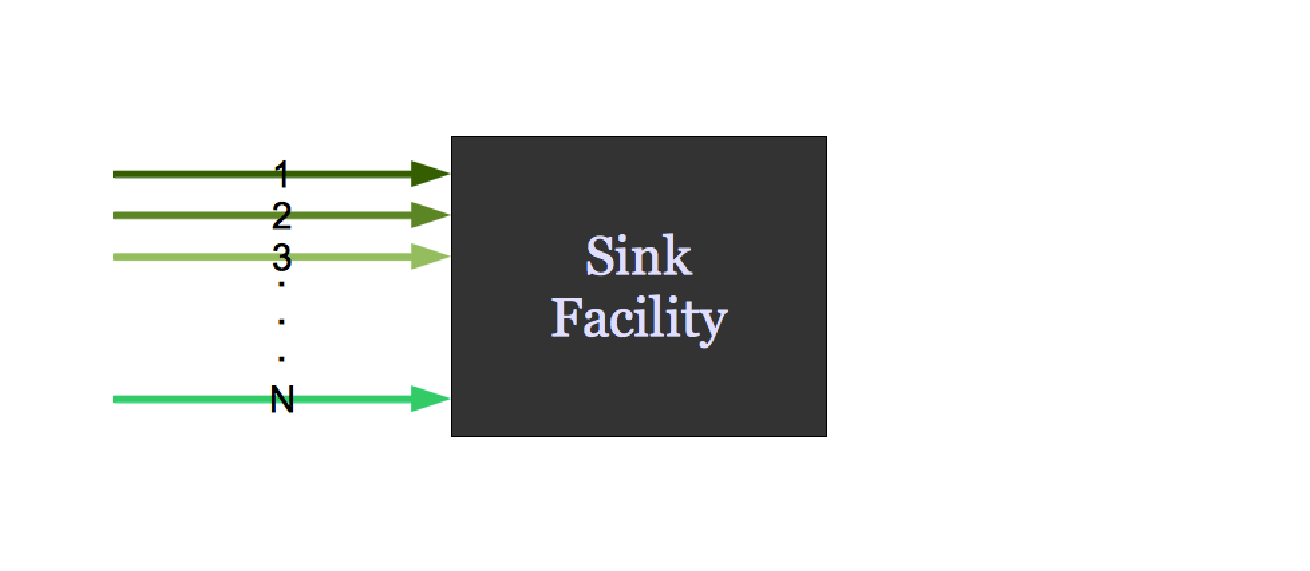
\includegraphics[height=5cm]{./images/sinkfacility.eps}
    \end{center}
    \caption{ To participate in a \Cyclus fuel cycle simulation, \Cyder must 
      accept \textbf{arbitrary} spent fuel and high level waste \textbf{material 
      data objects}.}
    \label{fig:sinkfacility}
  \end{figure}
% Sink Facility ?
\end{frame}

\begin{frame}[ctb!]
  \frametitle{Cyder Paradigm : Waste Stream Conditioning}
  \footnotesize{
  
\begin{figure}[htbp!]
\begin{center}
\def\svgwidth{.5\textwidth}
\input{./images/ws_conditioning.eps_tex}
\end{center}
\caption{In Cyder, discrete waste streams are conditioned into the appropriate 
discrete waste form according to user-specified pairings.}
\label{fig:ws_conditioning}
\end{figure}
}
\end{frame}

\begin{frame}[ctb!]
  \frametitle{Cyder Paradigm : Waste Form Packaging}
  \footnotesize{

\begin{figure}[htbp!]
\begin{center}
\def\svgwidth{.5\textwidth}
\input{./images/wf_packaging.eps_tex}
\end{center}
\caption{In Cyder, one or more waste forms are loaded into the appropriate 
waste package according to user-specified pairings.}
\label{fig:wf_packaging}
\end{figure}
}
\end{frame}

\begin{frame}[ctb!]
  \frametitle{Cyder Paradigm : Waste Package Emplacement}
\footnotesize{
  \begin{columns}[c]
    \column{0.3\linewidth}
Finally, the waste package is \textbf{emplaced} in a buffer component, which 
contains many other waste packages, spaced evenly in a grid. The grid is 
defined by the user input and depends on repository depth, $\Delta z$, waste 
package spacing, $\Delta x$, and tunnel spacing, $\Delta y$ as in Figure 
\ref{fig:repo_layout}.

    \column{0.6\linewidth}
\begin{figure}[htbp!]
\begin{center}
\def\svgwidth{.5\textwidth}
\input{./images/repo_layout.eps_tex}
\end{center}
\caption{The repository layout has a depth and a uniform package spacing.}
\label{fig:repo_layout}
\end{figure}
\end{columns}
  }
\end{frame}


\begin{frame}[ctb!]
  \frametitle{Cyder Paradigm : Modularity }
\begin{figure}[htbp!]
\begin{center}
\def\svgwidth{.6\textwidth}
\input{./images/modularity_layout.eps_tex}
\end{center}
%\caption{}
\label{fig:modularity_layout}
\end{figure}
\end{frame}


\begin{frame}[ctb!]
  \frametitle{Cyder Paradigm : Modularity }
\begin{figure}[htbp!]
\begin{center}
\def\svgwidth{.6\textwidth}
\input{./images/modularity_circle.eps_tex}
\end{center}
%\caption{}
\label{fig:modularity_circle}
\end{figure}
\end{frame}


\begin{frame}[ctb!]
  \frametitle{Cyder Paradigm : Modularity }
\begin{figure}[htbp!]
\begin{center}
\def\svgwidth{.6\textwidth}
\input{./images/modularity_colors.eps_tex}
\end{center}
%\caption{}
\label{fig:modularity_colors}
\end{figure}
\end{frame}


\begin{frame}
  \frametitle{Nested Components}
  Each Component has : 
  \begin{itemize}
    \item a Geometry to describe its dimensions and location
    \item a NuclideModel for contaminant transport 
    \item a ThermalModel for heat transport
    \item a Parent Component at its external barrier
    \item one or more Daughter Components at its internal barrier
  \end{itemize}

  Components have other data members such as a Type (WF, WP, BUFFER, FF), a 
  material data table, a start date, etc. 
\end{frame}

%\subsection{Cyder Models}
%\input{paradigm_models}
%\subsection{Cyder Data}
%\input{paradigm_data}

\section{Abstraction Methodology}


\begin{frame}[ctb!]
  \frametitle{Abstraction Methodology}
\footnotesize{
describe abstraction - thermal, radionuclide transport tools, sensitivity experiments, etc.

}
\end{frame}

\begin{frame}[ctb!]
  \frametitle{Abstraction Methodology}
\footnotesize{
abstraction methodology cont'd
}
\end{frame}

\subsection{Thermal Transport in Cyder}
\begin{frame}[ctb!]
\frametitle{Thermal Modeling in Cyder}
Two types of thermal modeling occur in Cyder. 
\begin{itemize}
\item The first is \textbf{capacity estimation} for waste stream acceptance.
\item The next is \textbf{heat evolution} which determines heat evolution in 
the modules over repository lifetime.
\end{itemize}
\end{frame}

\begin{frame}[ctb!]
\frametitle{Thermal Modeling in Cyder}
Each can be acheived with one thermal model,
\begin{itemize}
\item This model employs a Specific Temperature Change algorithm \cite{radel_effect_2007, radel_repository_2007} and
\item relies on a supporting \textbf{response database} combining detailed 
spent nuclear fuel composition data \cite{carter_fuel_2011} with a detailed 
thermal repository performance analysis tool from Lawrence Livermore National 
Lab (LLNL) and the Used Fuel Disposition (UFD) 
campaign \cite{greenberg_application_2012}.  
\item This method is capable of rapid estimation of temperature increase near emplacement tunnels as a function of 
\begin{itemize}
\item waste composition,
\item limiting radius, $r_{lim}$, 
\item waste package spacing, $S$, 
\item near field thermal conductivity, $K_{th}$, 
\item and near field thermal diffusivity, $\alpha_{th}$.
\end{itemize}
\end{itemize}
\end{frame}


\begin{frame}[ctb!]
\frametitle{Specific Temperature Change Method}
\footnotesize{
Introduced by Radel, Wilson et al., the Specific Temperature Change (STC) method uses 
a linear approximation to arrive at the thermal loading density limit 
\cite{radel_repository_2007, radel_effect_2007}.  

First, $\Delta T$ is determined for a limiting loading density 
of the particular material composition then it is normalized to a single 
kilogram of that material, $\Delta t$, the so called STC. 

\begin{align}
 \Delta T(r_{lim}) &= m \cdot \Delta t(r_{lim})
 \label{STC}
 \intertext{where}
 \Delta T &= \mbox{ Temperature change due to m }[K]\nonumber\\
 m &= \mbox{ Mass of heat generating material }[kg]\nonumber \\
 \Delta t &= \mbox{ Temperature change due to 1 kg }[K/kg]\nonumber\\
 r_{lim} &= \mbox{ Limiting radius } [m].\nonumber
\end{align}
}
\end{frame}

\begin{frame}[ctb!]
\frametitle{Specific Temperature Change Superposition}
\footnotesize{

For an arbitrary waste stream composition, scaled curves, $\Delta t_i$, calculated in this 
manner for individual isotopes can be superimposed for each isotope to arrive at an 
approximate total temperature change.

\begin{align}
 \Delta T (r_{lim}) &\sim \sum_{i} m_i \Delta t_i(r_{lim})
 \label{superposition}
\intertext{where}
 i &= \mbox{ An isotope in the material } [-]\nonumber\\
 m_i &= \mbox{ mass of isotope i  } [kg]\nonumber\\
 \Delta t_i &= \mbox{ Specific temperature change due to \textsl{i} } [K].\nonumber
\end{align}


}
\end{frame}

\subsubsection{Supporting Thermal Response Dataset}
To support this calculation in \Cyder, a reference data set of temperature change 
curves was calculated. Repeated runs of a detailed analytic model over the range of values in Table 
\ref{tab:thermal_cases} determined \gls{STC} values over a range of thermal 
heat limit radii, $r_{lim}$, thermal diffusivity values, $\alpha_{th}$,
thermal conductivity values, $K_{th}$ and waste package spacings, $S$. Linear 
interpolation across the discrete parameter space provides a simple thermal 
reference dataset for use in \Cyder.

\begin{table}[ht!]
\centering
\footnotesize{
\begin{tabular}{|l|l|l|r|}
\multicolumn{4}{c}{\textbf{Thermal Cases}}\\
\hline
\textbf{Parameter} & \textbf{Symbol} & \textbf{Units} & \textbf{Value Range} \\
\hline
Diffusivity & $\alpha_{th}$ & $[m^2\cdot s^{-1}]$ & $1.0\times10^{-7}-3.0\times10^{-6}$\\
\hline
Conductivity & $K_{th}$     & $[W\cdot m^{-1} \cdot K^{-1}]$ & $0.1 - 4.5$ \\
\hline
Spacing & $S$ & $[m]$ & 2, 5, 10, 15, 20, 25, 50 \\
\hline
Radius & $r_{lim}$ & $[m]$ & 0.1, 0.25, 0.5, 1, 2, 5 \\
\hline
Isotope & $i$ & $[-]$ & $^{241,243}Am,$  \\
        & & & $^{242,243,244,245,246}Cm,$  \\
        & & & $^{238,240,241,242}Pu$  \\
        & & & $^{134,135,137}Cs$  \\
        & & & $^{90}Sr$  \\
\hline
\end{tabular}
\caption{A thermal reference dataset of \gls{STC} values as a function of each of these parameters was generated by repeated parameterized runs of the LLNL 
MathCAD model\cite{greenberg_application_2012, greenberg_investigations_2012}.}
\label{tab:thermal_cases}
}
\end{table}



The analytic model used to populate the reference dataset was created at 
\gls{LLNL} for the \gls{UFD} campaign. In this tool, heat limited thermal 
response is calculated analytically for each geology, for many waste package 
loading densities, and for many fuel cycle options \cite{hardin_generic_2011, 
greenberg_investigations_2012, greenberg_application_2012}. It employs an 
analytic model from Carslaw and Jaeger and is implemented in MathCAD 
\cite{carslaw_conduction_1959, ptc_mathcad_2010}.  The integral solver in the 
MathCAD toolset is the primary calculation engine for the analytic MathCAD 
thermal model, which relies on superposition of point, finite-line, and line 
source integral solutions.  

%The transient state of the temperature at the calculation radius is found with a convolution of the transient far field solution with the steady state near field solution.  The process is then iterated with a one year resolution in order to arrive at a temperature evolution over the lifetime of the repository. 
%
%In a two dimensional grid of waste packages, the central package is represented by the finite line solution

Figure \ref{fig:CmScaling} demonstrates the scaling of an STC curve according to 
equation \eqref{STC} to represent the heat from $25.9g$ of initial $^{242}Cm$ using 
the reference data set. 

\begin{figure}[h!]
\begin{center}
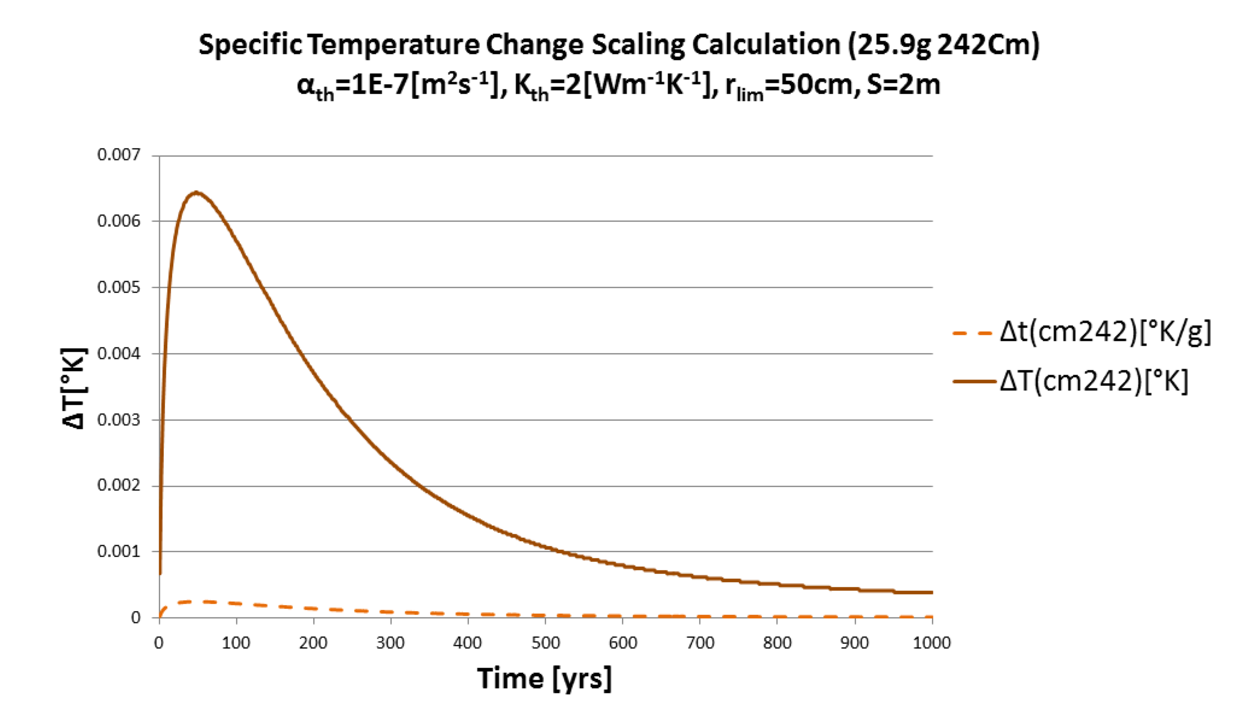
\includegraphics[width=\columnwidth]{./chapters/methodology/thermal_models/CmScaling.eps}
\end{center}
\caption{As a demonstration of the calculation procedure, the temperature change 
  curve for one initial gram of $^{242}Cm$ and is scaled to represent $25.9g$, 
  approximately the $^{242}Cm$ inventory per MTHM in 51GWd burnup UOX PWR fuel. }
\label{fig:CmScaling}
\end{figure}


The supporting database was limited to some primary heat contributing isotopes 
present in traditional spent nuclear fuel, $H$, 
such that the superposition in equation \eqref{superposition} becomes 

\begin{align}
\Delta T (r_{lim},S,K_{th},\alpha_{th})&\sim \sum_{i\in H} m_i \Delta t_i(r_{lim},S,K_{th},\alpha_{th})
\label{superposition_approx}
\intertext{where}
H &= \mbox{ set of high heat isotopes }[-]\nonumber\\
S &= \mbox{ uniform waste package spacing } [m]\nonumber\\
K_{th} &= \mbox{ thermal conductivity } [W\cdot m^{-1}\cdot K^{-1}]\nonumber\\
\alpha_{th} &= \mbox{ thermal diffusivity } [m^2\cdot s^{-1}]\nonumber\\
\end{align}

The use of this superposition is demonstrated in Figure 
\ref{fig:CmSuperposition}.

\begin{figure}[ht!]
\begin{center}
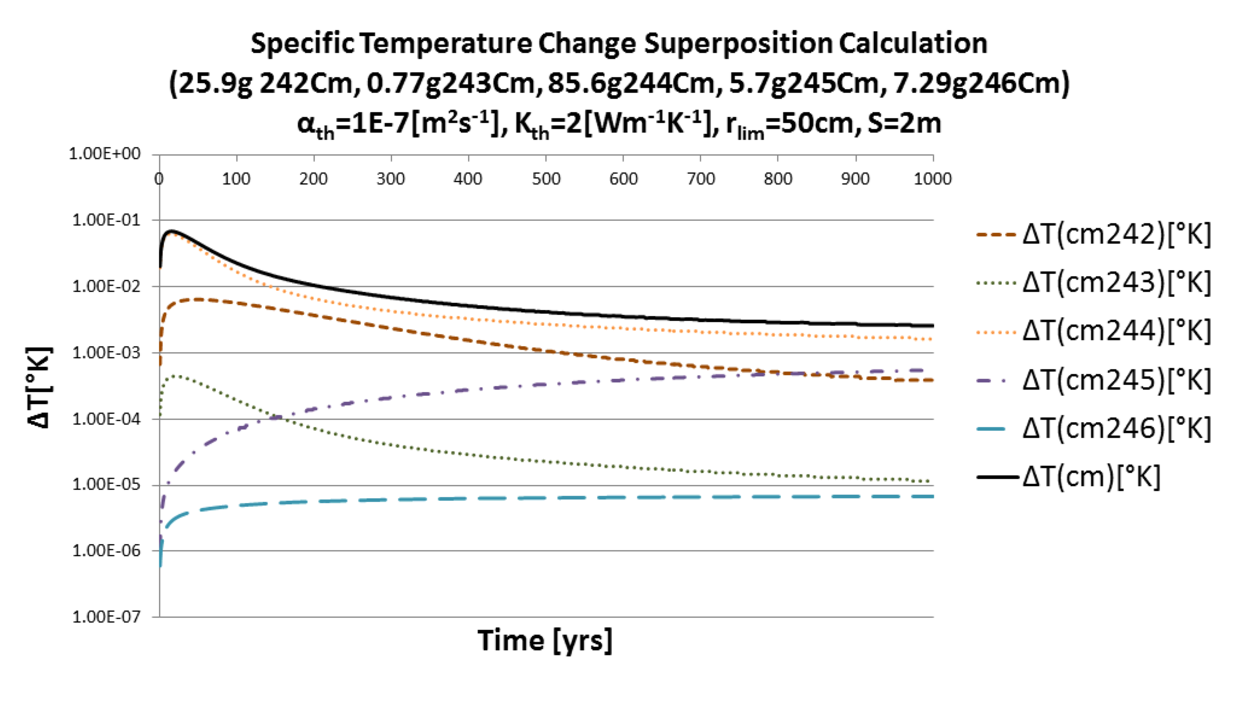
\includegraphics[width=\columnwidth]{./chapters/methodology/thermal_models/CmSuperposition.eps}
\end{center}
\caption{As a demonstration of the calculation procedure, scaled temperature change 
  curves for five curium isotopes are superimposed to achieve a total temperature 
change (note log scale).}
\label{fig:CmSuperposition}
\end{figure}

%\begin{align}
%  T_{line}(t,x,y,z) &= \frac{1}{8\pi K_{th}} 
%  \bigintsss_0^t\!\frac{q_L(t')}{t-t'}e^{ \frac{-\left(x^2 + z^2\right)}{4\alpha 
%  (t-t')} }\nonumber\\ &\cdot\left[ \erf{\left[ \frac{1}{2} \frac{\left( y + 
%  \frac{L}{2} \right)}{\sqrt{\alpha(t-t')}}  \right]} - \erf{\left[ \frac{1}{2} 
%  \frac{\left( y - \frac{L}{2} \right)}{\sqrt{\alpha(t-t')}}  \right]} 
%  \right]\,\mathrm{dt'},
%  \label{line}
%  \intertext{adjacent packages within the central tunnel are represented by the 
%  point source solution }
%  T_{point}(t,r) &= 
%  \frac{1}{8K_{th}\sqrt{\alpha}\pi^{\frac{3}{2}}}\bigintsss_0^{-t}\!\frac{q(t')}{(t-t')^{\frac{3}{2}}}e^{\frac{-r^2}{4\alpha(t-t')}}\,\mathrm{dt'},
%  \label{point}
%  \intertext{and adjacent disposal tunnels are represented by infinite line 
%  source solutions}
%  T_{\infty line}(t,x,z) &= \frac{1}{4\pi K_{th}} 
%  \bigintsss_0^t\!\frac{q_L(t')}{t-t'}e^{ \frac{-\left(x^2 + z^2\right)}{4\alpha 
%  (t-t')} }
%  \intertext{in infinite homogeneous media, where}
%  \label{infline}
%  \alpha &= ~~\mbox{thermal diffusivity } [m^2\cdot s^{-1}]\nonumber\\
%  q(t) &= ~~\mbox{point heat source} [W]\nonumber\\
%  \intertext{and}
%  q_L(t) &= ~~\mbox{linear heat source} [W\cdot m^{-1}]\nonumber
%\end{align}
%Superimposed point and line source solutions allow for a notion of the 
%repository layout to be modeled in the host rock.


\subsection{Radionuclide Transport in Cyder}
\begin{frame}
  \frametitle{Methodology Radionuclide Transport}
  nuclide transport models
\end{frame}


\section{Demonstration}
\begin{frame}
\frametitle{Demonstration}

\begin{itemize} 
\item Unit Testing Framework 
\item Base (Toy) Cases
\item Dominant Physics Validation Cases
\end{itemize}

\end{frame}

\subsection{Thermal Transport Toy Cases}

\begin{frame}[ctb!]
  \frametitle{Thermal Base Case Demonstration}
\begin{figure}[htp!]
\begin{center}
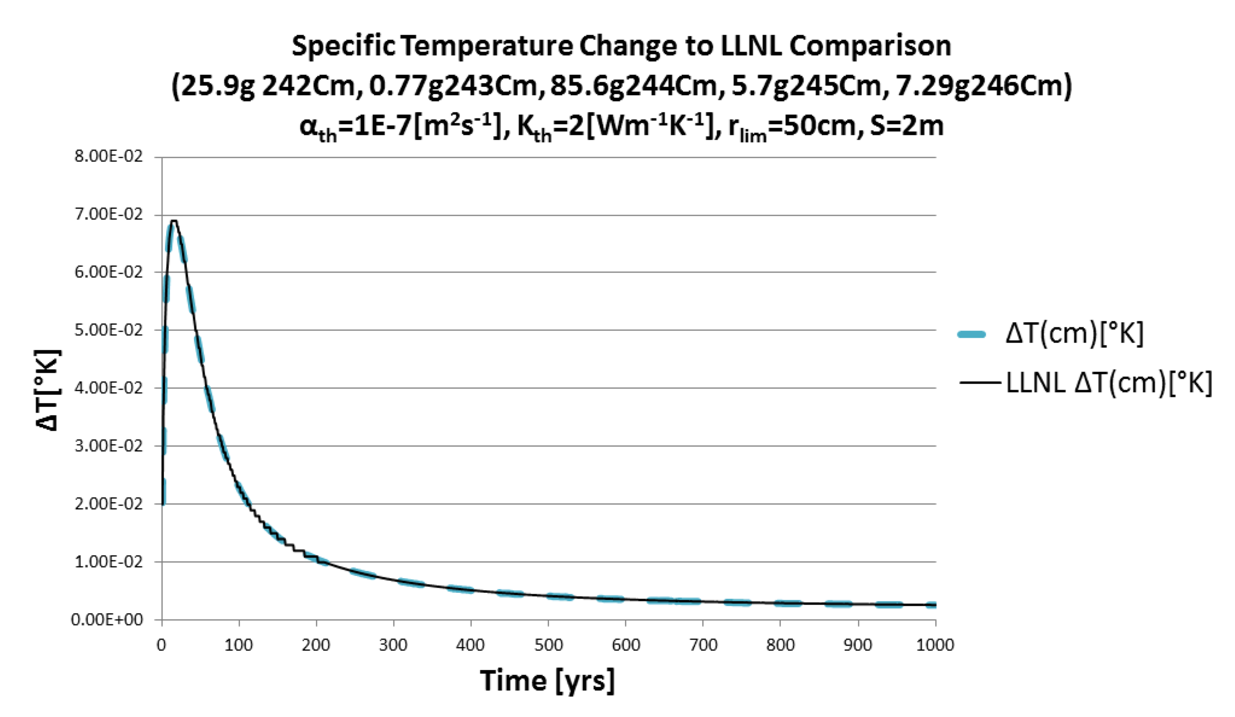
\includegraphics[width=\columnwidth]{./thermal_demonstration/CmValidation.eps}
\end{center}
\caption{This comparison of STC calculated thermal response from $Cm$ 
inventory per MTHM in 51GWd burnup UOX PWR fuel compares favorably with results 
from the semi-analytic model from LLNL.} 
\label{fig:CmValidation}
\end{figure}
\end{frame}


\begin{frame}[ctb!]
  \frametitle{Thermal Base Case Demonstration}
\begin{figure}[htp!]
\begin{center}
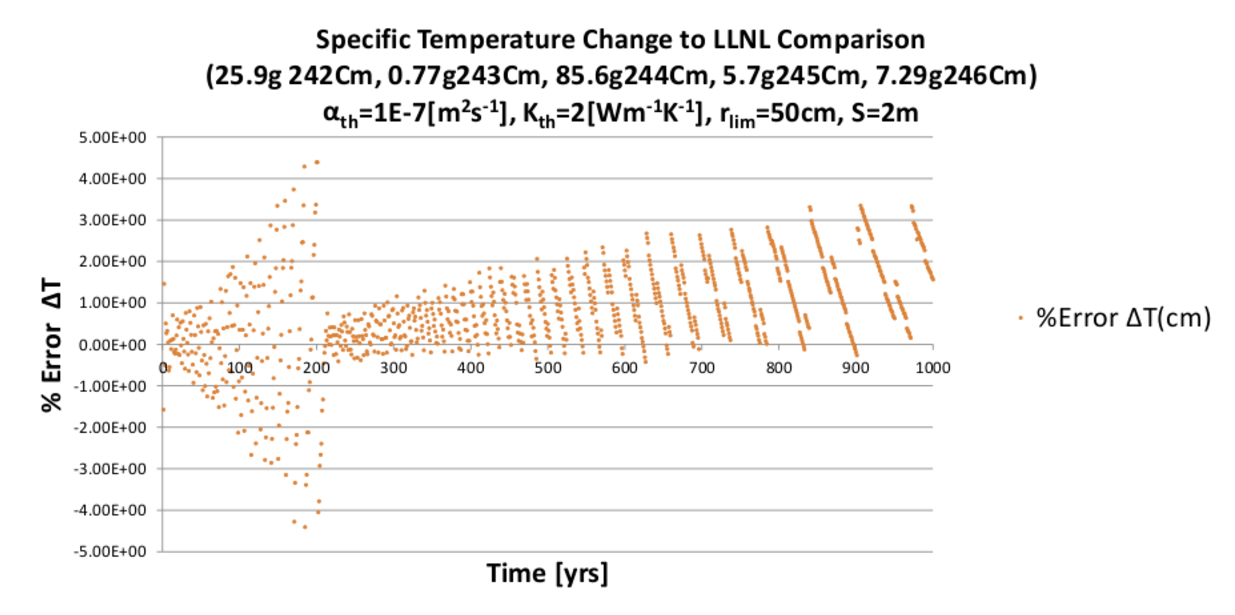
\includegraphics[width=\columnwidth]{./thermal_demonstration/CmPercentError.eps}
\end{center}
\caption{Percent error between the semi-analytic model from LLNL and the 
STC 
calculated thermal response from $Cm$ inventory per MTHM in 51GWd burnup UOX 
PWR fuel demonstrates a maximum percent error of 4.4\%.}
\label{fig:CmPercentError}
\end{figure}
\end{frame}


\subsection{Radionuclide Transport Toy Cases}
\begin{frame}[ctb!]
  \frametitle{Results Radionuclide Transport Base Cases}
\end{frame}


\begin{figure}[ht]
\centering
\includegraphics[width=0.6\textwidth]{./chapters/demonstration/base/drI.eps}
\caption[$^{235}U$ residence. Degradation Rate Waste Form No Release.]{
For Case DRI, in which total containment in the waste form is assumed ($F_{d,wf}=0$), 
$^{235}U$ takes up permanent residence in the waste form component.
}
\label{fig:drIall}
\begin{minipage}[b]{0.45\linewidth}

  \includegraphics[width=\textwidth]{./chapters/demonstration/base/drI1.eps}
  \caption[Case DRI Waste Form Contaminants.]{
    Waste Form 5 ($F_d = 0$) never releases material.
    }
  \label{fig:drIwf5}
  
  \includegraphics[width=\textwidth]{./chapters/demonstration/base/drI3.eps}
  \caption[Case DRI Buffer Contaminants]{
    The Buffer, component 7 ($F_d = 0.1$), never recieves material.
    }
  \label{fig:drIbuff}

\end{minipage}
\hspace{0.05\linewidth}
\begin{minipage}[b]{0.45\linewidth}
  \includegraphics[width=\textwidth]{./chapters/demonstration/base/drI2.eps}
  \caption[Case DRI Waste Package Contaminants.]{ 
    Waste Package 6 ($F_d = 0.1$), never recieves material.
    }
  \label{fig:drIwp6}

  \includegraphics[width=\textwidth]{./chapters/demonstration/base/drI0.eps}
  \caption[Case DRI Far Field Contaminants.]{ 
    The Far Field, component 0 ($F_d = 0.1$), never recieves material.
    }
  \label{fig:drIff0}

  \end{minipage}
\end{figure}
\FloatBarrier



\begin{figure}[ht]
\centering
\includegraphics[width=0.6\textwidth]{./chapters/demonstration/base/drII.eps}
\caption[$^{235}U$ residence. Degradation Rate Waste Package No Release.]{
For Case DRII, in which total containment in the waste package is assumed ($F_{d,wp}=0$), 
$^{235}U$ travels through waste forms ($F_d = 0.1$) before 
permanent residence in the waste package components.
}
\label{fig:drIIall}
\begin{minipage}[b]{0.45\linewidth}

  \includegraphics[width=\textwidth]{./chapters/demonstration/base/drII1.eps}
  \caption[Case DRII Waste Form Contaminants.]{
    Waste Form 5 ($F_d = 0.1$) releases material with degradation. 
    }
  \label{fig:drIIwf5}
  
  \includegraphics[width=\textwidth]{./chapters/demonstration/base/drII3.eps}
  \caption[Case DRII Buffer Contaminants]{
    The Buffer, component 7 ($F_d = 0.1$), never recieves material.
    }
  \label{fig:drIIbuff}

\end{minipage}
\hspace{0.05\linewidth}
\begin{minipage}[b]{0.45\linewidth}
  \includegraphics[width=\textwidth]{./chapters/demonstration/base/drII2.eps}
  \caption[Case DRII Waste Package Contaminants.]{ 
    Waste Package 6 ($F_d = 0$) acheives total containment.
    }
  \label{fig:drIIwp6}

  \includegraphics[width=\textwidth]{./chapters/demonstration/base/drII0.eps}
  \caption[Case DRII Far Field Contaminants.]{ 
    The Far Field, component 0 ($F_d = 0.1$), never recieves material.
    }
  \label{fig:drIIff0}


  \end{minipage}
\end{figure}
\FloatBarrier

\begin{figure}[ht]
\centering
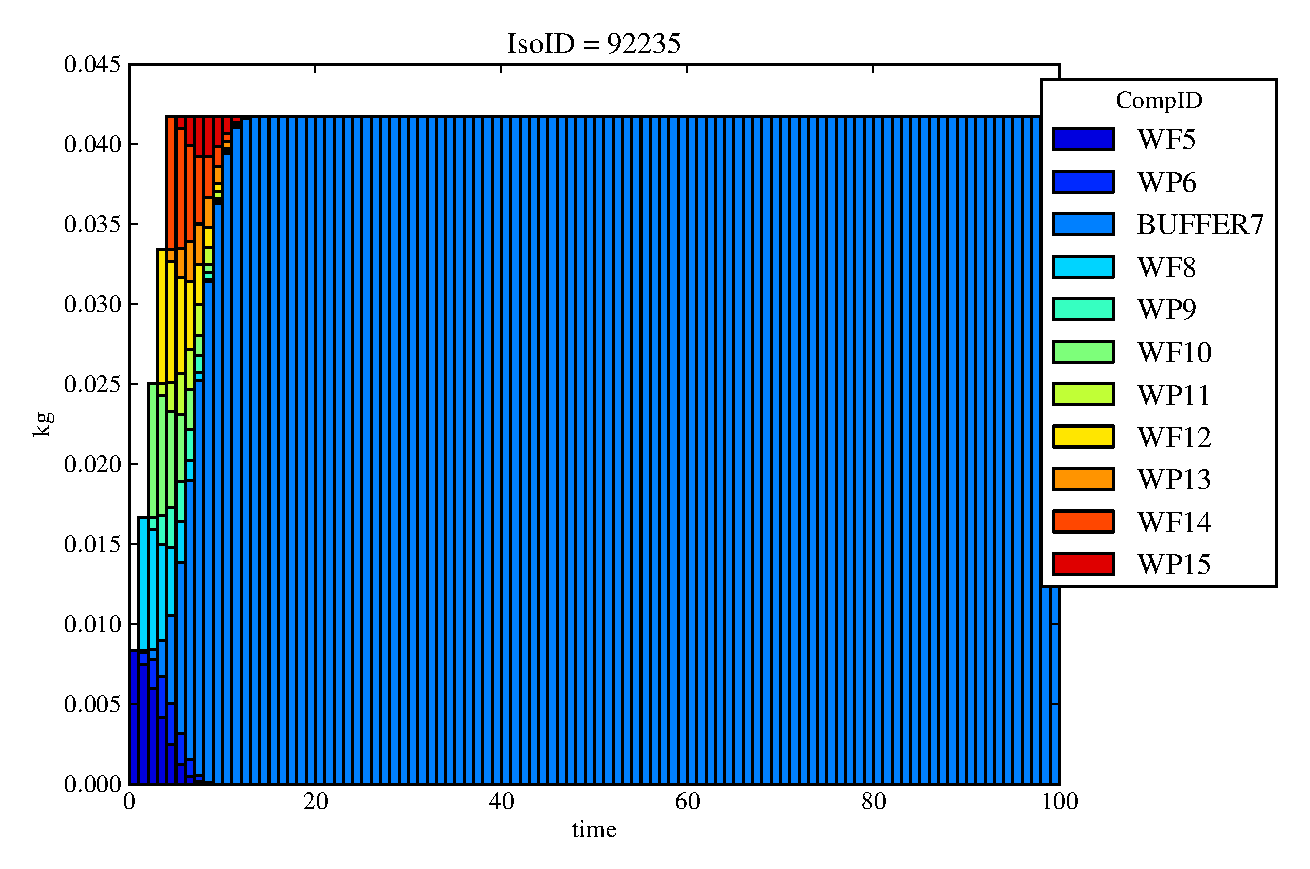
\includegraphics[width=0.6\textwidth]{./chapters/demonstration/base/drIII.eps}
\caption[$^{235}U$ residence. Degradation Rate Buffer No Release.]{
For Case DRIII, in which total containment in the buffer is assumed ($F_{d,buffer}=0$), 
$^{235}U$ travels through waste forms and waste package components ($F_d = 0.1$) before 
permanent residence in the buffer component.
}
\label{fig:drIIIall}
\begin{minipage}[b]{0.45\linewidth}

  \includegraphics[width=\textwidth]{./chapters/demonstration/base/drIII1.eps}
  \caption[Case DRIII Waste Form Contaminants.]{
    Waste Form 5 ($F_d = 0.1$) releases material with degradation. 
    }
  \label{fig:drIIIwf5}
  
  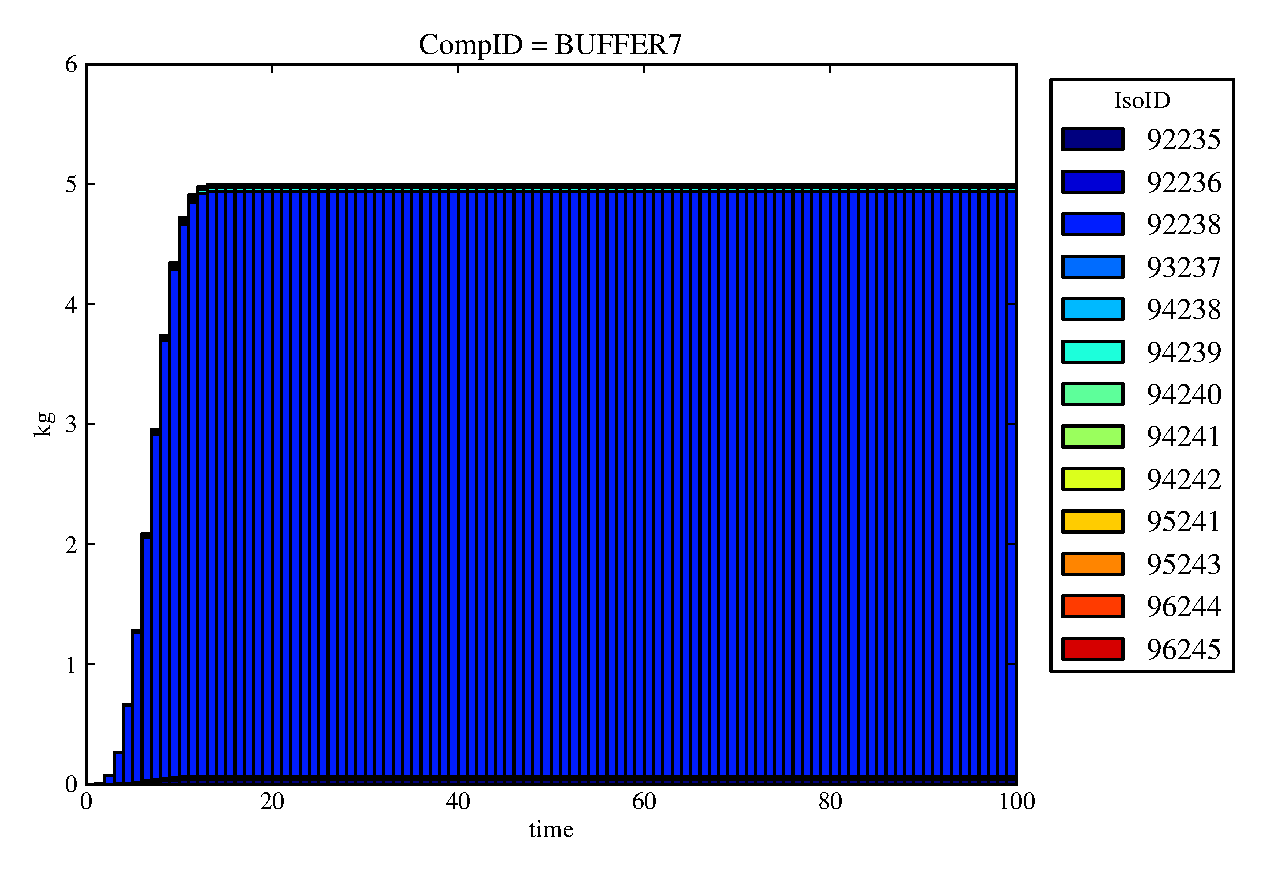
\includegraphics[width=\textwidth]{./chapters/demonstration/base/drIII3.eps}
  \caption[Case DRIII Buffer Contaminants]{
    The Buffer, component 7 ($F_d=0$), acheives total containment.
    }
  \label{fig:drIIIbuff}

\end{minipage}
\hspace{0.05\linewidth}
\begin{minipage}[b]{0.45\linewidth}
  \includegraphics[width=\textwidth]{./chapters/demonstration/base/drIII2.eps}
  \caption[Case DRIII Waste Package Contaminants.]{ 
    Waste Package 6 ($F_d = 0.1$) recieves then releases material. 
    }
  \label{fig:drIIIwp6}

  \includegraphics[width=\textwidth]{./chapters/demonstration/base/drIII0.eps}
  \caption[Case DRIII Waste Package Contaminants.]{ 
    The Far Field, component 0 ($F_d = 0.1$), never recieves material.
    }
  \label{fig:drIIIff0}


  \end{minipage}
\end{figure}
\FloatBarrier



\begin{figure}[ht]
\centering
\includegraphics[width=0.6\textwidth]{./chapters/demonstration/base/drIV.eps}
\caption[$^{235}U$ residence. Degradation Rate Buffer No Release.]{
For DRIV case in which total containment in the far field is assumed ($F_{d,ff}=0$), 
$^{235}U$ travels through interior components ($F_d = 0.1$) before 
permanent residence in the far field component.
}
\label{fig:drIVall}
\begin{minipage}[b]{0.45\linewidth}

  \includegraphics[width=\textwidth]{./chapters/demonstration/base/drIV1.eps}
  \caption[Case DRIV Waste Form Contaminants.]{
    Waste Form 5 ($F_d = 0.1$) releases material with degradation. 
    }
  \label{fig:drIVwf5}
  
  \includegraphics[width=\textwidth]{./chapters/demonstration/base/drIV3.eps}
  \caption[Case DRIV Buffer Contaminants]{
    The Buffer, component 7 ($F_d=0.0$), receives and then releases material.
    }
  \label{fig:drIVbuff}

\end{minipage}
\hspace{0.05\linewidth}
\begin{minipage}[b]{0.45\linewidth}
  \includegraphics[width=\textwidth]{./chapters/demonstration/base/drIV2.eps}
  \caption[Case DRIV Waste Package Contaminants.]{ 
    Waste Package 6 ($F_d = 0.1$) recieves then releases material. 
    }
  \label{fig:drIVwp6}

  \includegraphics[width=\textwidth]{./chapters/demonstration/base/drIV0.eps}
  \caption[Case DRIV Waste Package Contaminants.]{ 
    The Far Field, component 0 ($F_d = 0.0$), acheives total containment.
    }
  \label{fig:drIVff0}


  \end{minipage}
\end{figure}


\begin{frame}[ctb!]
  \frametitle{Mixed Cell Model Base Case I}
\begin{figure}[ht]
\centering
\includegraphics[width=0.8\textwidth]{./images/mcI.eps}
\caption[$^{235}U$ residence. Mixed Cell Sorption Limitation Without Solubility Limitation.]{
For the MCI case in which total containment is only is assumed in the far field, 
but sorption and solubility limitation neglected, demonstrates results exactly similar to 
DRIV, as expected.}
\label{fig:mcI}
\end{figure}
\end{frame}

\begin{frame}[ctb!]
  \frametitle{Mixed Cell Model Base Case I}
  \begin{figure}[htbp!]
\begin{minipage}[b]{0.45\linewidth}

  \includegraphics[width=0.8\textwidth]{./images/mcI1.eps}
  \caption[MCI Waste Form Contaminants.]{
    Waste Form 5 ($F_d = 0.1$) releases material with degradation. 
    }
  \label{fig:mcIwf5}
  
  \includegraphics[width=0.8\textwidth]{./images/mcI3.eps}
  \caption[Case MCI Buffer Contaminants]{
    Buffer 7 ($F_d=0.1$), receives and releases material.
    }
  \label{fig:mcIbuff}

\end{minipage}
\hspace{0.05\linewidth}
\begin{minipage}[b]{0.45\linewidth}
  \includegraphics[width=0.8\textwidth]{./images/mcI2.eps}
  \caption[Case MCI Waste Package Contaminants.]{ 
    Waste Package 6 ($F_d = 0.1$) receives and releases material.
    }
  \label{fig:mcIwp6}

  \includegraphics[width=0.8\textwidth]{./images/mcI0.eps}
  \caption[Case MCI Waste Package Contaminants.]{ 
    Far Field 4 ($F_d = 0.0$) acheives full containment.
    }
  \label{fig:mcIff0}


  \end{minipage}
\end{figure}
\end{frame}

\begin{frame}[ctb!]
  \frametitle{Mixed Cell Model Base Case II}
\begin{figure}[ht]
\centering
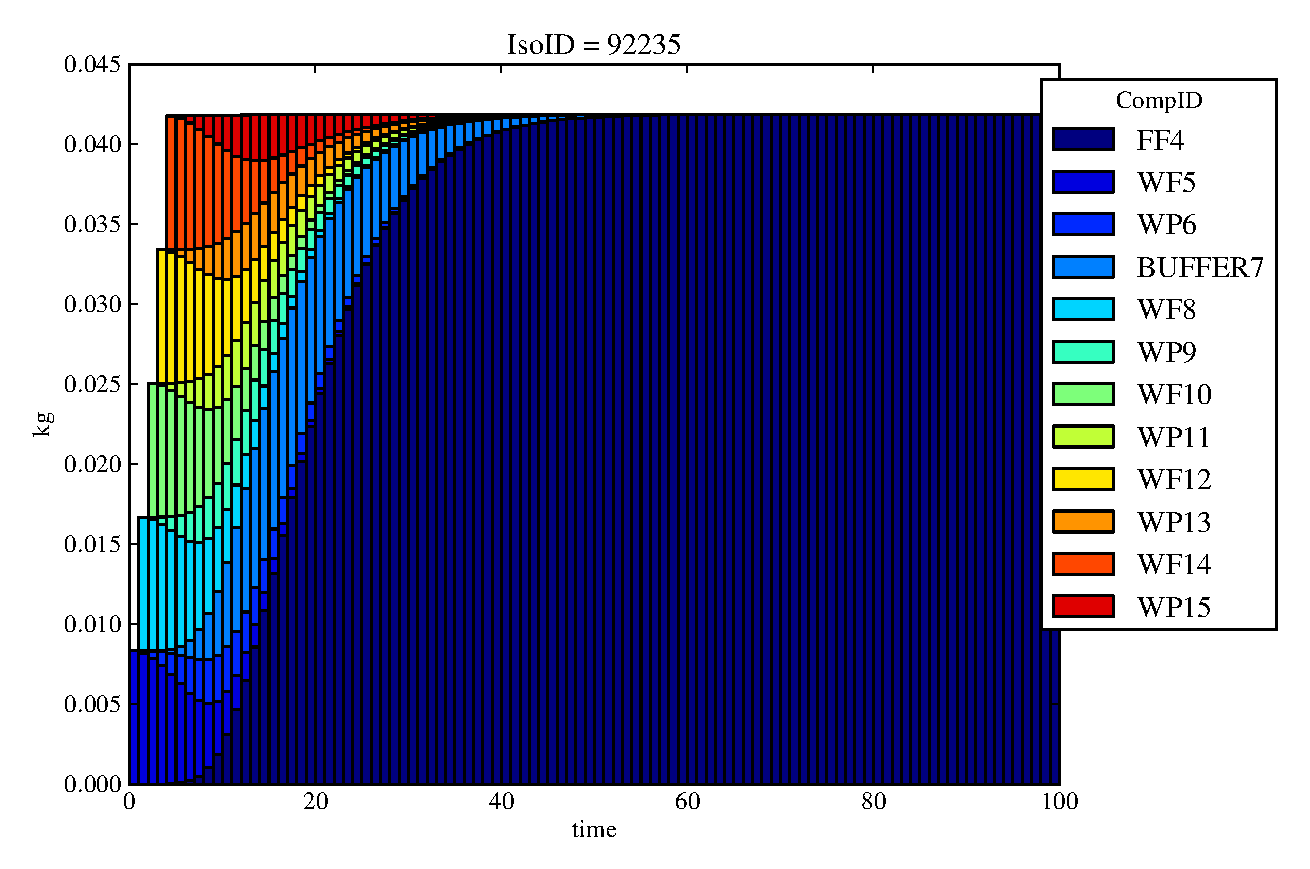
\includegraphics[width=0.8\textwidth]{./images/mcIII.eps}
\caption[$^{235}U$ residence. Mixed Cell Coupled Sorption and Solubility Limitation.]{
For the MCII case in which containment is affected by both sorption and 
solubility limitation,
($F_{d}=0.1$ for all components), $^{235}U$ travels more slowly than in the MCI case 
before permanent residence in the far field component.
}
\label{fig:mcIIIall}
\end{figure}
\end{frame}

\begin{frame}[ctb!]
  \frametitle{Mixed Cell Model Base Case II}
  \begin{figure}
\begin{minipage}[b]{0.45\linewidth}

  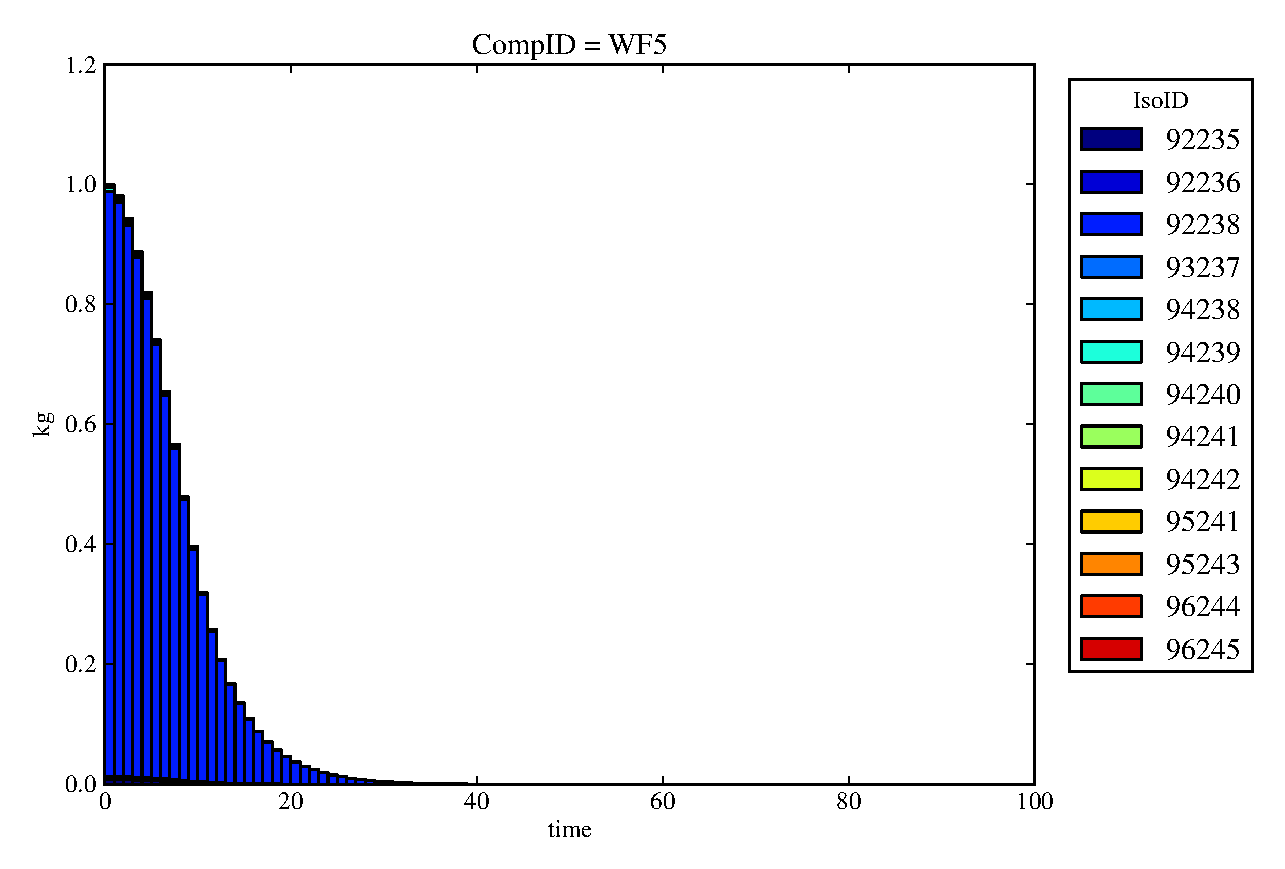
\includegraphics[width=0.8\textwidth]{./images/mcIII1.eps}
  \caption[MCI Waste Form Contaminants.]{
    Waste Form 5 ($F_d = 0.1$) releases material with degradation. 
    }
  \label{fig:mcIIIwf5}
  
  \includegraphics[width=0.8\textwidth]{./images/mcIII3.eps}
  \caption[Case MCI Buffer Contaminants]{
    Buffer 7 ($F_d=0.1$), receives and releases material.
    }
  \label{fig:mcIIIbuff}

\end{minipage}
\hspace{0.05\linewidth}
\begin{minipage}[b]{0.45\linewidth}
  \includegraphics[width=0.8\textwidth]{./images/mcIII2.eps}
  \caption[Case MCI Waste Package Contaminants.]{ 
    Waste Package 6 ($F_d = 0.1$) receives and releases material. 
    }
  \label{fig:mcIIIwp6}

  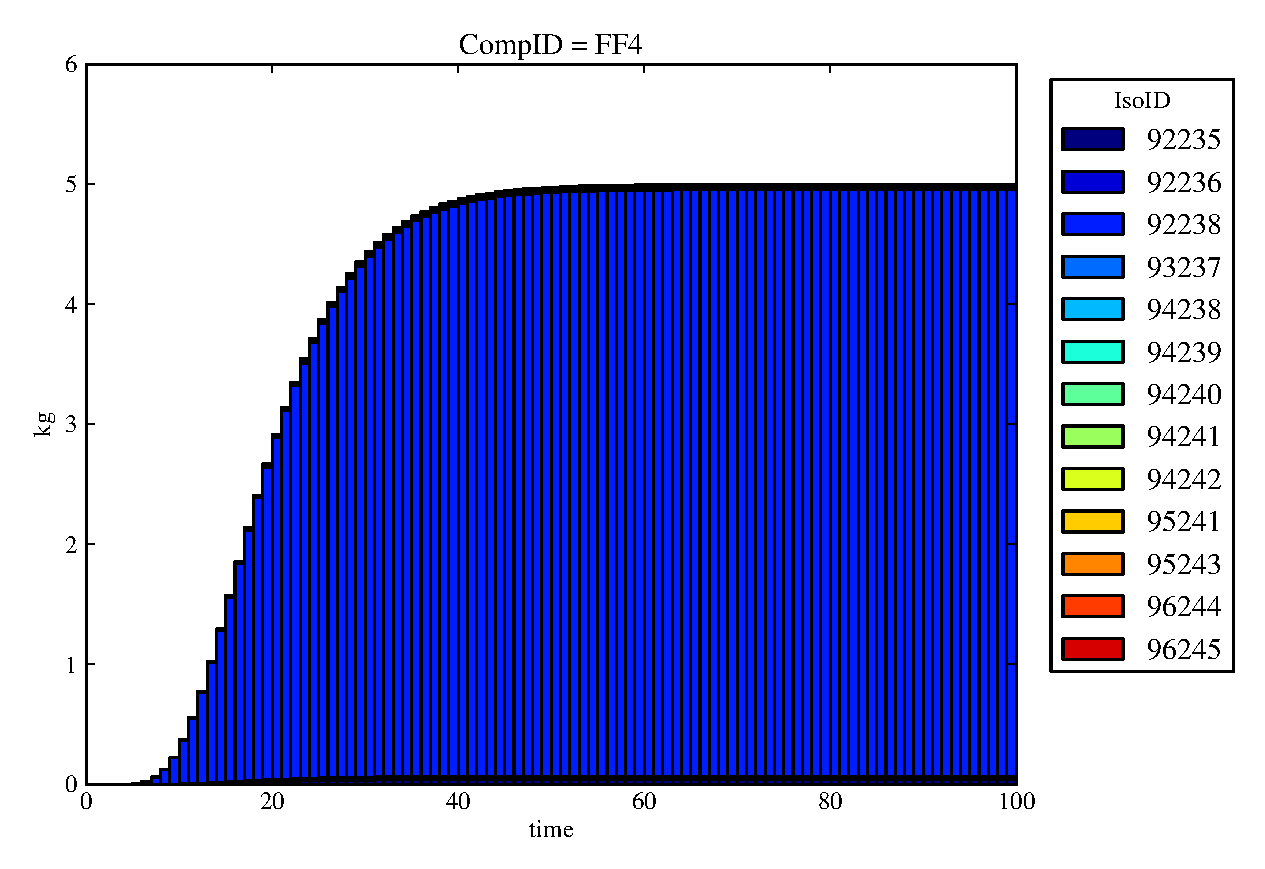
\includegraphics[width=0.8\textwidth]{./images/mcIII0.eps}
  \caption[Case MCI Waste Package Contaminants.]{ 
    Far Field 4 ($F_d = 0.1$) acheives total containment.
    }
  \label{fig:mcII}


  \end{minipage}
\end{figure}

\end{frame}


\subsection{Thermal Transport Validation Cases}

\section{Spacing Thermal Transport Sensitivity Studies}\label{sec:spacing}



\begin{frame}[ctb!]
\frametitle{LLNL Model Thermal Conductivity Sensitivity}
By varying the thermal conductivity of the repository model from 0.1 to 4.5 
$[W\cdot m^{-1} \cdot K^{-1}]$, this sensitivity analysis succeeds in capturing 
the domain of thermal conductivities witnessed in high thermal conductivity 
salt deposits as well as low thermal conductivity clays.


\begin{figure}[htbp!]
\begin{center}
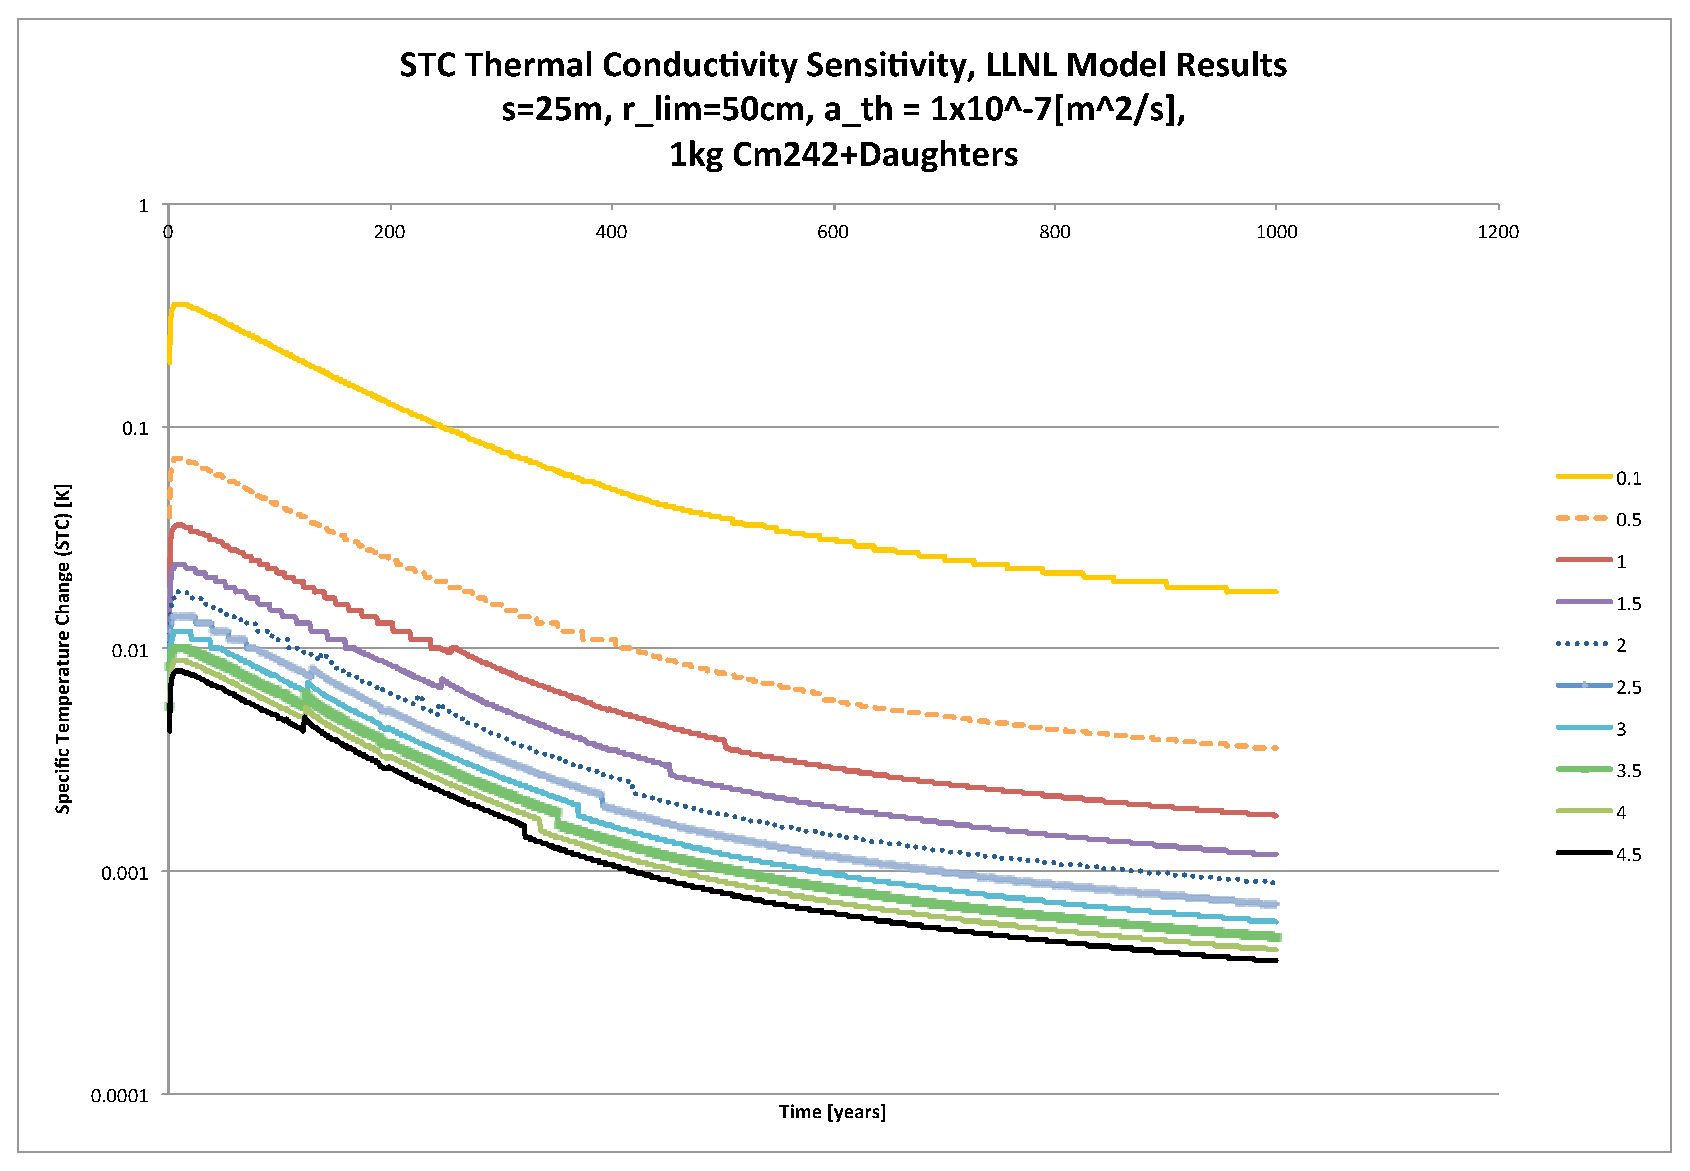
\includegraphics[height=0.7\textheight]{./thermal_demonstration/conductivity/Cm242kth_alpha_low.eps}
\end{center}
\caption[$K_{th}$ Sensitivity for Low $\alpha_{th}$ in LLNL Model]{Increased thermal conductivity decreases thermal energy deposition 
(here represented by STC) in the near field (here $r_{calc} = 0.5m$).}
\label{fig:Cm242Kth_alpha_low}
\end{figure}

\end{frame}


\begin{frame}[ctb!]
\frametitle{Cyder Thermal Conductivity and Limiting Radius Sensitivity}

Figures \ref{fig:kr} and \ref{fig:ks} validate the trend noted above that 
increased thermal conductivity of a medium decreases thermal energy deposition 
in the near field. Additionally, analysis with the \Cyder STC database 
demonstrates the way in which the importance of spacing and the importance of 
the limiting radius decrease with increasing $K_{th}$.

\begin{figure}[htbp!]
\begin{center}
\includegraphics[height=0.7\textheight]{./thermal_demonstration/conductivity/kr.eps}
\end{center}
\caption[$K_{th}$ vs. $r_{lim}$ Sensitivity in Cyder]
{Cyder results agree with 
those of the LLNL model. The importance of the limiting radius decreases with 
increased $K_{th}$. The above example thermal profile results from 10kg of 
$^{242}Cm$}
\label{fig:kr}
\end{figure}
\end{frame}

\begin{frame}[ctb!]
\frametitle{Cyder Thermal Conductivity and Limiting Radius Sensitivity}

\begin{figure}[htbp!]
\begin{center}
\includegraphics[height=0.7\textheight]{./thermal_demonstration/conductivity/ks.eps}
\end{center}
\caption[$K_{th}$ vs. Waste Package Spacing Sensitivity in Cyder]{Cyder results agree with 
those of the LLNL model. The importance of the limiting radius decreases with 
increased $K_{th}$. The above example thermal profile results from 10kg of 
$^{242}Cm$}
\label{fig:ks}
\end{figure}
\end{frame}




\subsection{Diffusion Coefficient of Far Field}
\label{sec:diffusivity}

In clay media, diffusion dominates far field hydrogeologic transport due to 
characteristically low hydraulic head gradients and permeability. Thus, the effective diffusion 
coefficient is a parameter to which repository performance in clay media is 
expected to be very sensitive. 

The sensitivity of the peak dose to the reference diffusivity of the 
host rock was analyzed.  In this model, the reference diffusivity of the medium 
was the input parameter used to vary the effective diffusivity in a controlled 
manner. In GoldSim's transport module, the effective diffusion coefficient is 
defined as 

\begin{align}\label{diffcoeff}
  D_{eff} &= n\tau D_{ref}D_{rel} \\ % ?  
       D_{eff} &= ~~\mbox{effective diffusion coefficient }[m^2/s],\nonumber\\
       D_{rel} &= ~~\mbox{relative diffusivity for each isotope in water }[\%],\nonumber\\
       D_{ref} &= ~~\mbox{reference diffusivity in water }[m^2/s],\nonumber\\
       \tau &= ~~\mbox{tortuosity} [\%], \nonumber \\ 
       n &= ~~\mbox{porosity}[\%].\nonumber\\
  \label{GDSEdiff}
\end{align}

The reference diffusivity was altered while the porosity and the tortuosity 
were both set to 1. Thus, the simulation rendered the effective diffusivity 
equal to the product of the reference diffusivity and the relative diffusivity 
(set to 1 for all isotopes).  This allowed the diffusivity to be controlled 
directly for all isotopes.

The waste inventory total mass was also altered for each value of the reference 
diffusivity.  That is, the radionuclide inventory in a reference 
\gls{MTHM} of commercial spent nuclear fuel was multiplied by a scalar mass factor.  
It was expected that changing these two parameters in tandem would capture the 
importance of diffusivity in the far field to the repository performance 
as well as a threshold at which the effect of waste inventory dissolution is 
attenuated by solubility limits.

Finally, in order to isolate the effect of the far field behavior, the waste form 
degradation rate was set to be very high as were the solubility and advective 
flow rate through the  \gls{EBS}. This guaranteed that contaminant flowthrough 
in the near field was unhindered, leaving the far field as the dominant barrier 
to release.


\subsubsection{Parametric Range}
\label{sec:diffCoeffRange}

The forty runs corresponded to eight values of relative diffusivity and five 
values of inventory mass multiplier. That is, the reference diffusivity was varied over the 
eight magnitudes between $ 10^{-8}$ and $10^{-15}$ $[m^2 /s]$ . 
The Mass Factor, the unitless inventory multiplier, was simultaneously varied over 
the five magnitudes between $10^{-4}$ and $10^{1} [-]$. That is, the 
radionuclide inventory was varied between $10^{-4}$ and $10^{1}$ of that in one 
\gls{MTHM} of \gls{SNF}, which is expected to cover the full range of 
inventories in current wasteforms.

\begin{table}[hbp!]
\centering
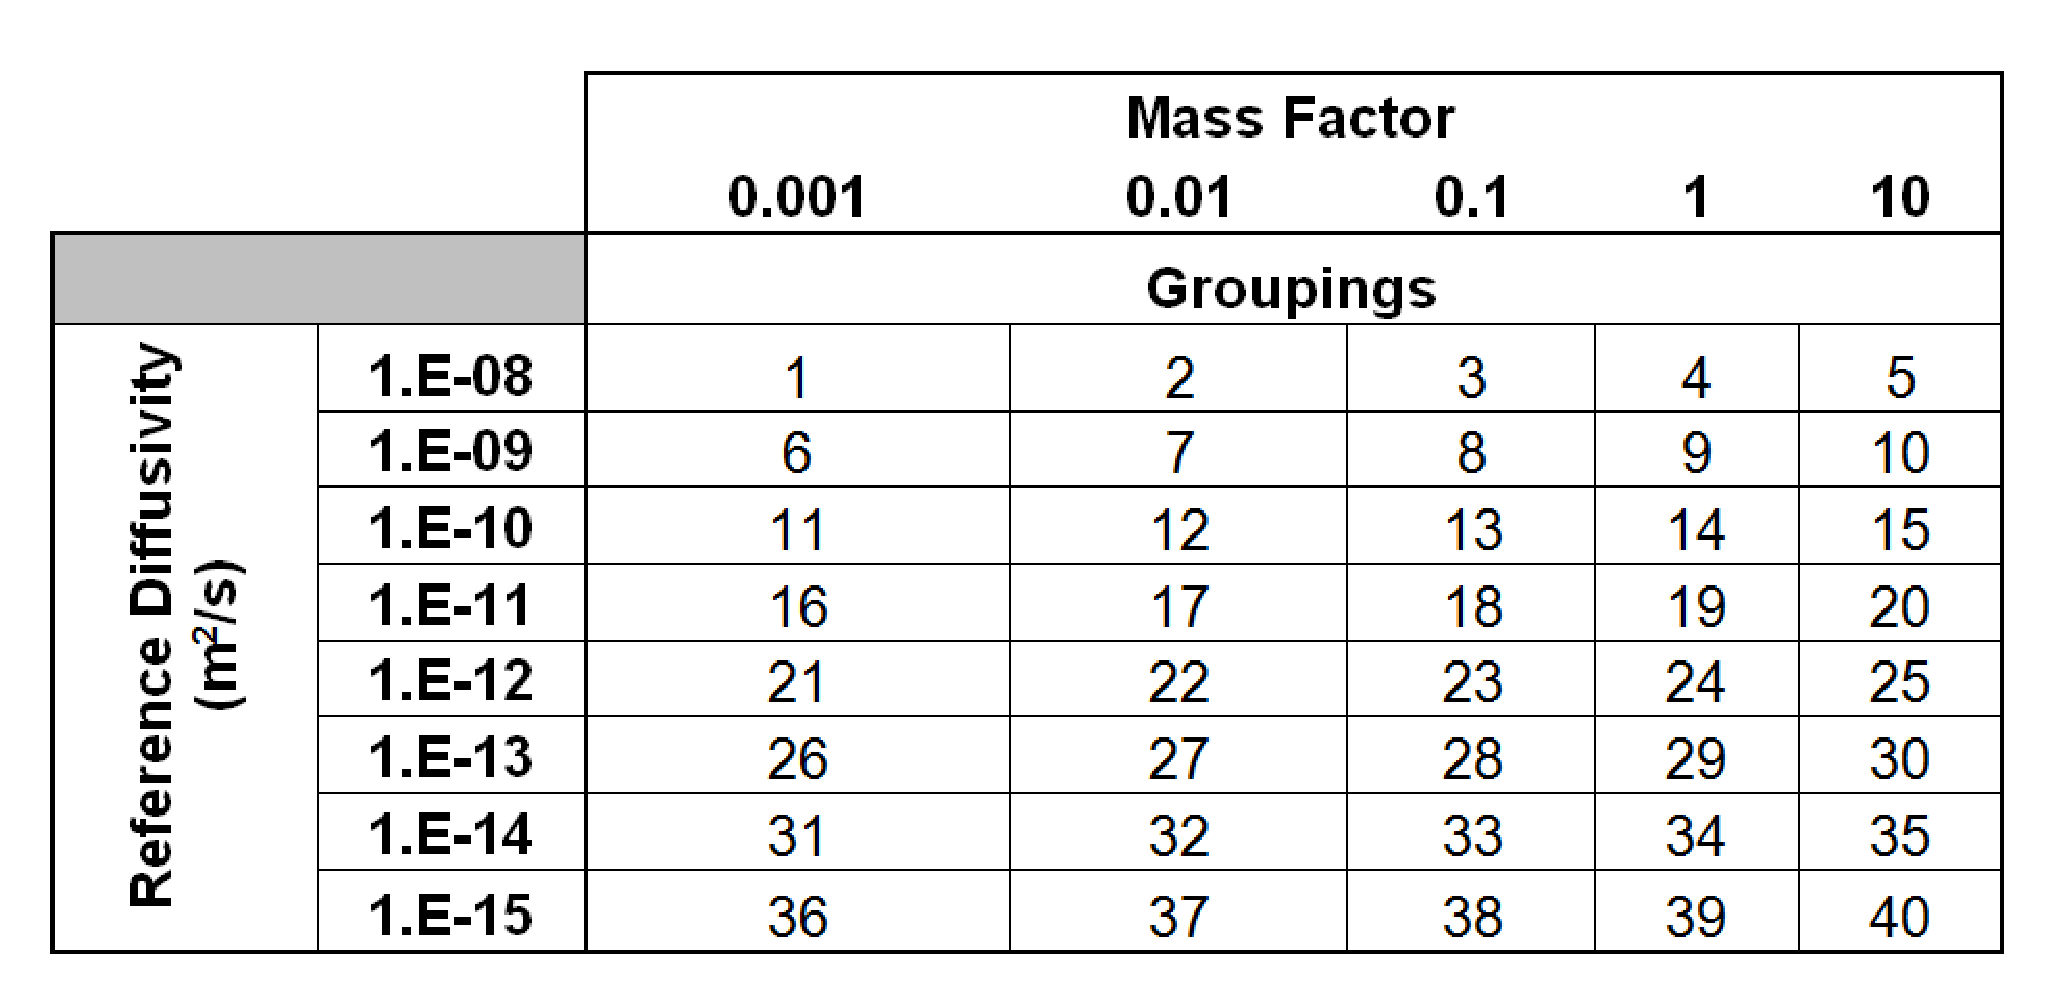
\includegraphics[width=0.7\textwidth]{./chapters/nuclide_sensitivity/clay/DiffCoeffAndInvEBSFail/DiffCoeffAndInvGroups.eps}
\caption{Diffusion coefficient and mass factor simulation groupings.}
\label{tab:DiffCoeffAndInvGroups}
\end{table}

\subsubsection{Results}


The peak doses due to highly soluble, non-sorbing elements such as $I$ and $Cl$, 
are  proportional to the radionuclide inventory and 
largely directly proportional to the relative diffusivity. This can be seen for 
the cases of $^{129}I$ and $^{36}Cl$ in Figures \ref{fig:DCInvI129}, 
\ref{fig:DCInvI129MF}, \ref{fig:DCInvCl36} and \ref{fig:DCInvCl36MF}.

\begin{figure}[ht]
\centering
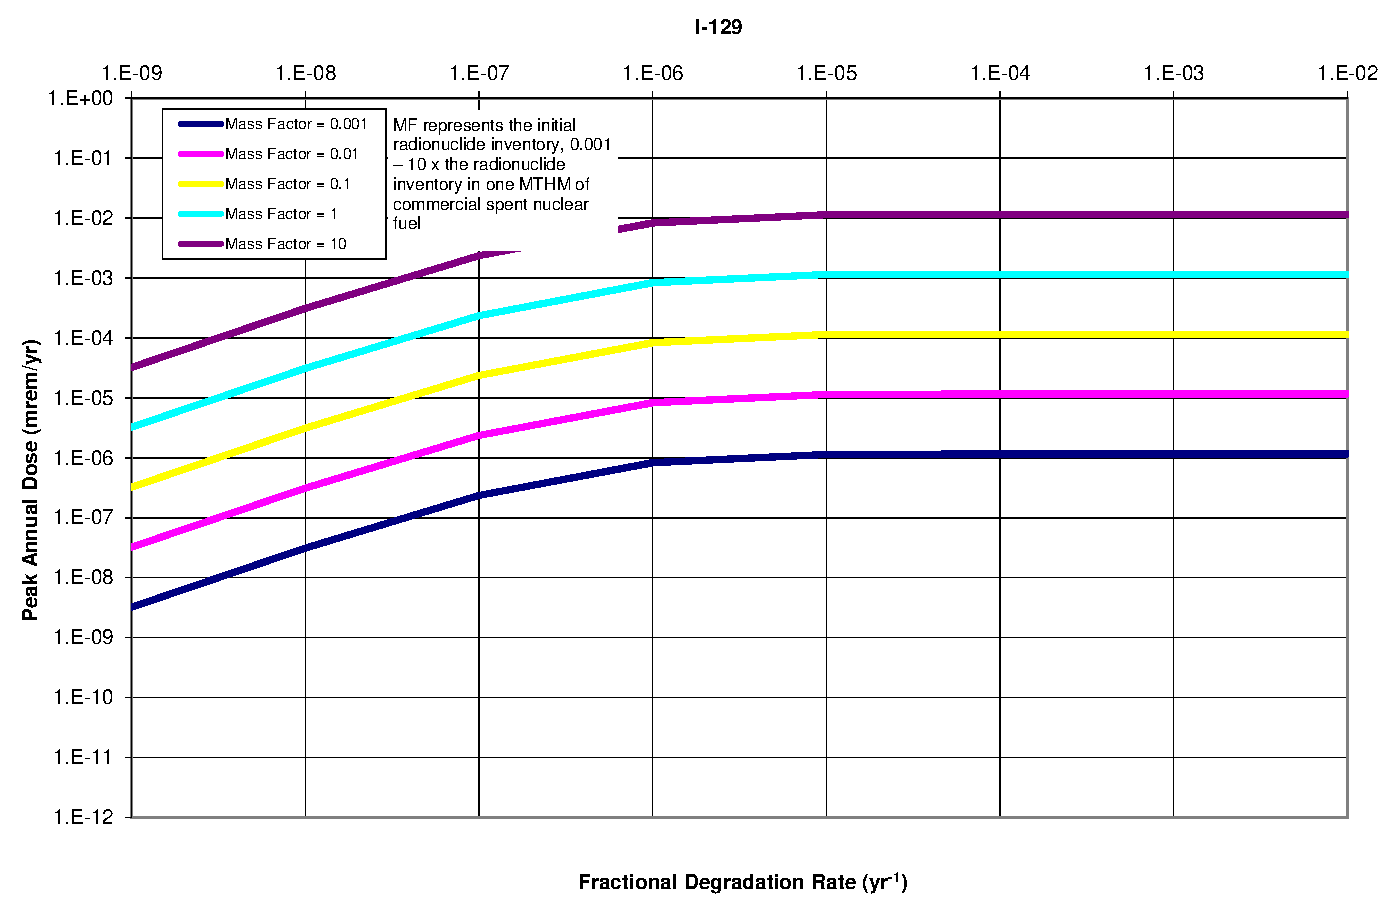
\includegraphics[width=\linewidth]{./chapters/nuclide_sensitivity/clay/DiffCoeffAndInvEBSFail/I-129.eps}
\caption{$^{129}I$ relative diffusivity sensitivity.}
\label{fig:DCInvI129}
\end{figure}

\begin{figure}[ht]
\centering
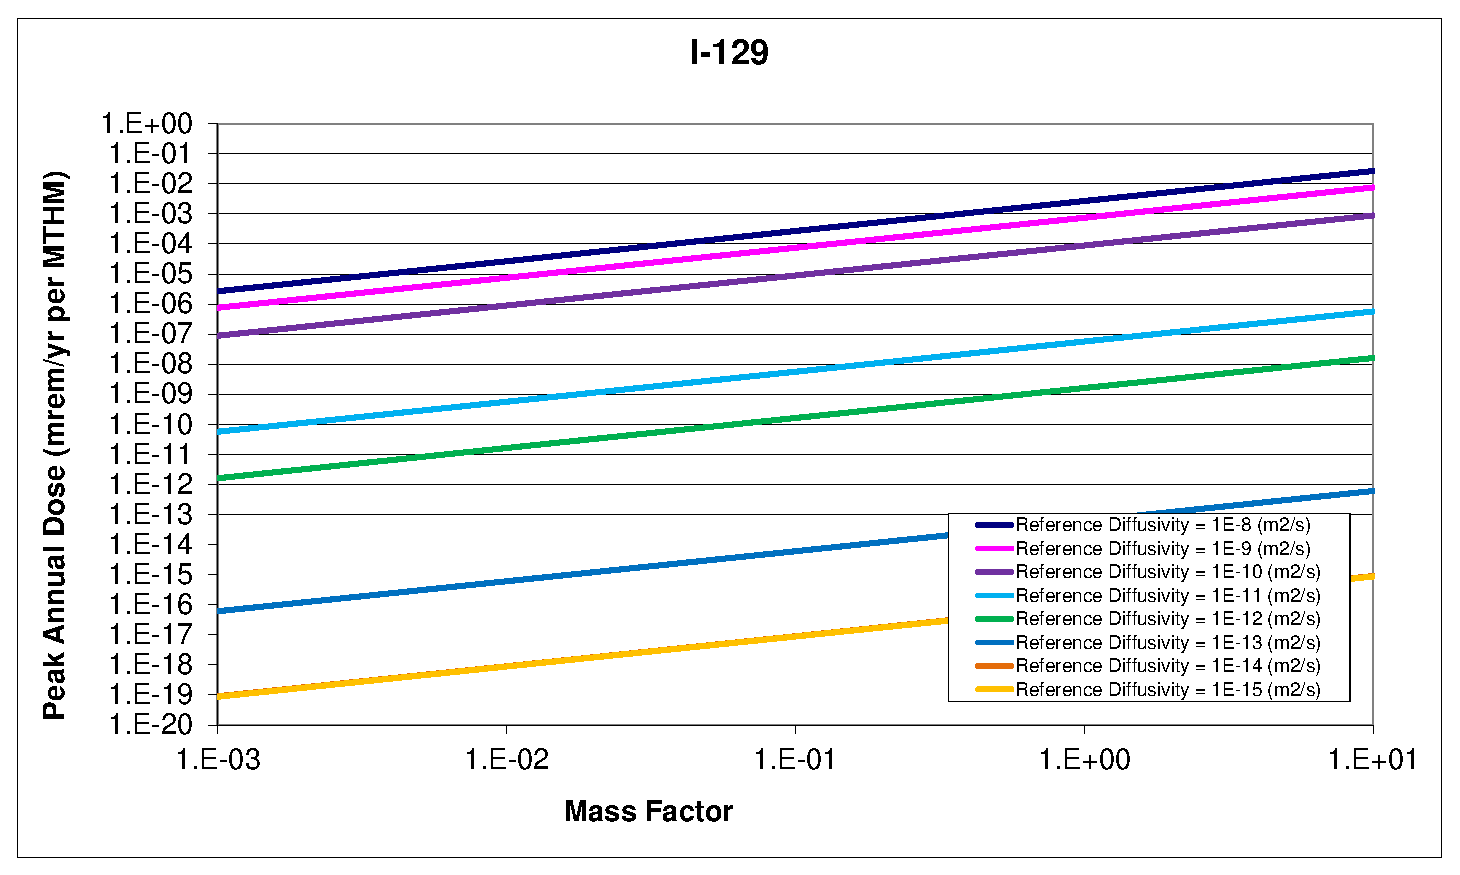
\includegraphics[width=\linewidth]{./chapters/nuclide_sensitivity/clay/DiffCoeffAndInvEBSFail/I-129-MF.eps}
\caption{$^{129}I$ mass factor sensitivity.}
\label{fig:DCInvI129MF}
\end{figure}

\begin{figure}[ht]
\centering
\includegraphics[width=\linewidth]{./chapters/nuclide_sensitivity/clay/DiffCoeffAndInvEBSFail/Cl-36.eps}
\caption{$^{36}Cl$ relative diffusivity sensitivity.}
\label{fig:DCInvCl36}
\end{figure}

\begin{figure}[ht]
\centering
\includegraphics[width=\linewidth]{./chapters/nuclide_sensitivity/clay/DiffCoeffAndInvEBSFail/Cl-36-MF.eps}
\caption{$^{36}Cl$ mass factor sensitivity.}
\label{fig:DCInvCl36MF}
\end{figure}

Long lived $^{129}I$ and $^{36}Cl$ are assumed to have near complete solubility, 
so in Figures \ref{fig:DCInvI129} and \ref{fig:DCInvCl36}, the effect of a 
solubility limited attenuation regime is not seen. Even for very low 
diffusivities, the diffusion length of the far field is the primary barrier. In 
Figures \ref{fig:DCInvI129MF} and \ref{fig:DCInvCl36MF} it is clear that in the 
absence of solubility limitation and sorption, the peak dose is directly 
proportional to mass factor. 

Both $Cl$ and $I$ are soluble and non-sorbing. The amount of $^{129}I$ in the 
\gls{SNF} inventory is greater than the amount of $^{36}Cl$, so a difference in 
magnitudes are expected, however, the trends should be the same. Since the 
halflife of $^{36}Cl$, $3\times10^5[yr]$, is much shorter than the half life of 
$^{129}I$, $1.6\times10^7[yr]$, a stronger proportional dependence on mass 
factor is seen for $Cl$ due to its higher decay rate. 

With the exception of those dose-contributors assumed to be completely soluble, 
two regimes were visible in the results of this analysis. In low diffusion 
coefficient regime, the diffusive pathway through the homogeneous permeable 
porous medium in the far field continues to be a  dominant barrier to nuclide 
release for normal (non-intrusive) repository conditions. 

In the second regime, for very high diffusion coefficients, the effects of 
additional attenuation phenomena in the natural system can be seen.  The 
dependence of peak annual dose on mass factor was consistently directly 
proportional for all isotopic groups.

The peak doses due to solubility limited, sorbing elements such as $Np$ and 
$Tc$ demonstrate two major regimes. In the first regime, for 
low values of mass factor, the mean of the peak annual dose rates is directly 
proportional to both reference diffusivity and mass factor.  For higher values 
of mass factor, the sensitivity to reference diffusivity and mass factor are 
both attenuated at higher values.  The attenuation in these regimes 
is due to natural system attenuation, most notably, sorption.

$^{237}Np$ and $^{99}Tc$ exhibit a strong proportional relationship 
between diffusivity and dose in Figures \ref{fig:DCInvTc99} and 
\ref{fig:DCInvNp237}. This relationship is muted as diffusivity 
increases. Both are directly proportional to mass factor until they reach the 
point of attenuation by their solubility limits, as can be seen in 
Figures \ref{fig:DCInvTc99MF} and \ref{fig:DCInvNp237MF}.

\begin{figure}[ht!]
\centering
\includegraphics[width=\linewidth]{./chapters/nuclide_sensitivity/clay/DiffCoeffAndInvEBSFail/Tc-99.eps}
\caption{$^{99}Tc$ relative diffusivity sensitivity.} 
\label{fig:DCInvTc99}
\end{figure}

\begin{figure}[ht!]
\centering
\includegraphics[width=\linewidth]{./chapters/nuclide_sensitivity/clay/DiffCoeffAndInvEBSFail/Tc-99-MF.eps}
\caption{$^{99}Tc$ mass factor sensitivity.}
\label{fig:DCInvTc99MF}
\end{figure}


\begin{figure}[ht!]
\centering
\includegraphics[width=\linewidth]{./chapters/nuclide_sensitivity/clay/DiffCoeffAndInvEBSFail/Np-237.eps}
\caption{$^{237}Np$ relative diffusivity sensitivity.} 
\label{fig:DCInvNp237}
\end{figure}

\begin{figure}[ht!]
\centering
\includegraphics[width=\linewidth]{./chapters/nuclide_sensitivity/clay/DiffCoeffAndInvEBSFail/Np-237-MF.eps}
\caption{$^{237}Np$ mass factor sensitivity.}
\label{fig:DCInvNp237MF}
\end{figure}



\clearpage








\subsection{Radionuclide Transport Validation Cases}

\begin{frame}[ctb!]
\frametitle{Cyder Advective Diffusive Threshold}
\input{./nuclide_demonstration/sol_sensitivity}
\input{./nuclide_demonstration/sol_results}

\end{frame}

\begin{frame}[ctb!]
\frametitle{Cyder Advective Diffusive Threshold}
\input{./chapters/demonstration/bench/kd_sensitivity}

\end{frame}

\begin{frame}[ctb!]
\frametitle{Cyder Advective Diffusive Threshold}
\input{./nuclide_demonstration/wf_deg_inv_sensitivity}
\input{./nuclide_demonstration/wf_deg_inv_results}

%\subsection{Case IVI : Waste Package Failure Time and Diffusion Coefficient Sensitivity}
%\input{./chapters/demonstration/bench/wpfail_diff_sensitivity}

\end{frame}

\begin{frame}[ctb!]
\frametitle{Cyder Advective Diffusive Threshold}

\input{./nuclide_demonstration/adv_vel_diff_sensitivity}
\input{./nuclide_demonstration/adv_vel_diff_results}

\end{frame}



\section{Conclusion}
\chapter{Conclusions}\label{ch:conclusion}
\section{Contributions}

This work has provided a flexible code for rapid medium fidelity calculation of 
generic repository performance in the context of fuel cycle analysis.  Capable 
of thermal transport, hydrologic contaminant transport, and integration 
within a fuel cycle simulation code, \Cyder is the first of its kind.  

In addition to implementing fundamental modeling capabilities, \Cyder has been 
designed to accommodate the development of advanced capabilities in the future.

In this work, key conceptual components and modeling methods for geologic 
radioactive waste disposal were identified as part of a literature review, 
dominant physics of thermal and radionuclide transport were identified by 
conducting sensitivity analyses with detailed codes. Accordingly, a basic set 
of abstracted models were developed and implemented within the \Cyder code. 

A set of basic capabilities within the \Cyder library have been developed and 
validated and an assortment of advanced features, data, testing, and plotting 
capabilities are functional.  The \Cyder source code in which these models are 
implemented  is made freely available to interested researchers and potential 
model developers \cite{huff_cyder_2013}. In addition to the source code and 
supporting publications, the \Cyder code is well commented and produces 
clickable, browsable automated documentation with each build. That 
documentation is also available online.

The application programming interface to this software library is intentionally 
general, facilitating the incorporation of the models presented here within 
external software tools in need of a multicomponent disposal system simulator. 

Furthermore, this work contributes to an expanding ecosystem of computational 
models available for use with the \Cyclus fuel cycle simulator. This hydrologic 
nuclide transport library, by virtue of its capability to modularly integrate 
with the \Cyclus fuel cycle simulator has laid the foundation for integrated 
disposal option analysis in the context of fuel cycle options. 

\section{Suggested Future Work}
It is hoped that \Cyder will benefit from continued development and use. Future 
development efforts will likely be led by developer use cases, but are likely 
to include a number of advanced features that have the potential to extend the 
capabilities of this tool in significant ways. 

Initially, further validation of these models should include full benchmarks 
against the \gls{GDSM} results including biosphere conversion of the released 
source term.  Furthermore, thermal benchmarks against recent \gls{UFD} work for 
various design concepts would similarly improve the understanding of the range 
of validity for the thermal model. 

Thermal analysis in these results have been used to assess thermal performance 
of a repository after emplacement. However, dynamic, thermal capacity limited 
fuel cycle analyses concerning the variation of necessary cooling times among 
repository concepts and fuel cycles should be conducted using the capacity 
determination capability arrived at with this model.  

Additional advanced capabilities should include the incorporation of fracture 
enabled transport in a radionuclide transport model. This feature would improve 
analyses of geologic host media such as granite which exhibit significant 
cracking. Similarly, incorporation of a biosphere model in the far field would 
substantively benefit the calculation of fuel cycle metrics related to human and 
environmental effects and will support myriad expected use cases of the tool.

Additional radionuclide transport models, thermal transport models, and 
supporting data will enrich the capabilities of this code. 


%%--------------------------------%%
%%--------------------------------%%
\begin{frame}[allowframebreaks]
  \frametitle{References}
  \bibliographystyle{plain}
  {\footnotesize \bibliography{defense} }

\end{frame}

%%--------------------------------%%


\appendix
\newcounter{finalframe}
\setcounter{finalframe}{\value{framenumber}}


\begin{frame}[ctb!]
\frametitle{GDSM Model Advective Diffusive Sensitivity}

\begin{figure}[htp!]
\begin{minipage}[b]{0.45\linewidth}
\centering
\includegraphics[width=\linewidth]{./nuclide_demonstration/AdvVelDiff/I-129.eps}
\caption{$^{129}I$ reference diffusivity sensitivity.}
\label{fig:VAdvVelI129}

\end{minipage}
\hspace{0.05\linewidth}
\begin{minipage}[b]{0.45\linewidth}

\includegraphics[width=\linewidth]{./nuclide_demonstration/AdvVelDiff/I-129-VAdvVel.eps}
\caption{$^{129}I$ vertical advective velocity sensitivity.}
\label{fig:VAdvVelI129VAdvVel}

\end{minipage}
\end{figure}
\end{frame}


\subsubsection{Advection vs. Diffusion Sensitivity Cyder Results}
Some of the  radionuclide transport models in \Cyder depend on the advective velocity as well as the diffusion 
characteristics of the medium. By evaluating the sensitivity to the advective velocity and reference 
diffusivity of the radionuclide transport in the MixedCell model, trends similar to those found in the \gls{GDSM} were found with the \Cyder tool. 
Specifically, increased advection and increased diffusion lead to greater release. Also, when both are varied, a boundary between diffusive and advective
regimes can be seen. An example of these results are shown in Figure \ref{fig:mixed_adv_diff}.
 
\begin{figure}[ht]
\centering
%\includegraphics[width=\linewidth]{./chapters/demonstration/bench/mixed_diff.eps}
\caption[Advection vs. Diffusion Sensitivity in Cyder]{Dual advective velocity 
and reference diffusivity sensitivity for a non-sorbing, infinitely soluble 
nuclide.}
\label{fig:mixed_adv_diff}
\end{figure}


\section{LLNL Model Background}
% LLNL
\subsection{Analytical Model Background}
\begin{frame}[ctb!]
\frametitle{Analytical Model : Background}
The analytical  model
\begin{itemize} 
  \item was created at LLNL (H. Greenberg, J. Blink, et. al) \cite{hardin_generic_2011, sutton_investigations_2011, 
greenberg_application_2012}
  \item employs an analytic model from Carslaw and Jaeger \cite{carslaw_conduction_1959} 
  \item is implemented in MathCAD \cite{ptc_mathcad_2010}
  \item seeks to inform heat limited waste capacity calculations for 
    \begin{itemize}
      \item arbitrary geology 
      \item arbitrary waste package loading densities
      \item arbitrary homogeneous decay heat source
    \end{itemize}
\end{itemize}
\end{frame}

\begin{frame}
  \frametitle{Analytical Model : Geometry}
  \begin{figure}[h!]
    \begin{center}
      \includegraphics[width=0.7\textwidth]{./images/llnlConcept.eps}
    \caption{Vertical, horizontal, alcove, and borehole emplacement layouts can 
    be represented by a line of point sources and adjacent line sources 
    \cite{sutton_investigations_2011}.}
    \label{fig:llnl}
    \end{center}
  \end{figure}
\end{frame}

\begin{frame}
  \frametitle{Analytical Model : Calculation Method}
    LLNL's model is a MathCAD solution of the transient homogeneous 
    conduction equation,
    \begin{align}
      \nabla^2T  = \frac{1}{\alpha}\frac{\partial T}{\partial t},
      \label{condGl}
    \end{align}
    in which superimposed point and line source solutions approximate the repository 
    layout.
\end{frame}

\begin{frame}[ctb!]
\frametitle{Analytical Model : Calculation Method}
The model consists of two conceptual regions, an external region representing 
the host rock and an internal region representing the waste form, package, and 
buffer Engineered Barrier System within the disposal tunnel wall.   
\begin{itemize}
  \item Since the thermal mass of the EBS is small in comparison to the thermal 
    mass of the host rock, the internal region may be treated as quasi-steady 
    state.
  \item The transient state of the temperature at the calculation radius is 
    found with a convolution of the transient external solution with the steady 
    state internal solution.
  \item The internal and external regions are \textbf{approximated} to be a 
    single homogeneous medium.
  \item The process is then iterated with a one year resolution in order to 
    arrive at a temperature evolution over the lifetime of the repository. 
\end{itemize}
\end{frame}


\begin{frame}[ctb!]
\frametitle{Analytical Model : Calculation Method}
\begin{minipage}{0.3\textwidth}
\begin{figure}[h!]
  \begin{center}
    \includegraphics[width=\textwidth]{./images/llnlConcept.eps}
  \end{center}
  \caption{The central package is represented by a finite line source
  \cite{sutton_investigations_2011}.}
  \label{fig:llnl}
\end{figure}
\end{minipage}
\hspace{0.01mm}
\begin{minipage}{0.6\textwidth}
The geometric layout of the analytic LLNL model in Figure \ref{fig:llnl} 
shows  that the central package is represented by the finite line solution
\footnotesize{
\begin{align}
  T_{line}&(t,x,y,z) = \nonumber\\
  &\frac{1}{8\pi K_{th}} 
  \bigintsss_0^t\!\frac{q_L(t')}{t-t'}e^{ \frac{-\left(x^2 + z^2\right)}{4\alpha 
  (t-t')} }\nonumber\\ &\cdot\left[ \erf{\left[ \frac{1}{2} \frac{\left( y + 
  \frac{L}{2} \right)}{\sqrt{\alpha(t-t')}}  \right]} - \erf{\left[ \frac{1}{2} 
  \frac{\left( y - \frac{L}{2} \right)}{\sqrt{\alpha(t-t')}}  \right]} 
  \right]\,\mathrm{dt'}.
  \label{line}
\end{align}
}
\end{minipage}
\end{frame}

\begin{frame}[ctb!]
\frametitle{Analytical Model : Calculation Method}
\begin{minipage}{0.3\textwidth}
\begin{figure}[h!]
  \begin{center}
    \includegraphics[width=\textwidth]{./images/llnlConcept.eps}
  \end{center}
  \caption{Adjacent packages are represented as point sources
  \cite{sutton_investigations_2011}.}
  \label{fig:llnl}
\end{figure}
\end{minipage}
\hspace{0.1mm}
\begin{minipage}{0.6\textwidth}
 Adjacent packages within the central tunnel are represented by the point source 
 solution,
 \footnotesize{
  \begin{align}
    T_{point}(t,r) &= \frac{1}{8K_{th}\sqrt{\alpha}\pi^{\frac{3}{2}}}\nonumber\\
     &\bigintsss_0^{t}\!\frac{q(t')}{(t-t')^{\frac{3}{2}}}e^{\frac{-r^2}{4\alpha(t-t')}}\,\mathrm{dt'}.
    \label{point}
  \end{align}
  }
  \end{minipage}
\end{frame}


\begin{frame}[ctb!]
\frametitle{Analytical Model : Calculation Method}
\begin{minipage}{0.3\textwidth}
\begin{figure}[h!]
  \begin{center}
    \includegraphics[width=\textwidth]{./images/llnlConcept.eps}
  \end{center}
  \caption{The non-central disposal tunnels are represented as infinite line sources
  \cite{sutton_investigations_2011}.}
  \label{fig:llnl}
\end{figure}
\end{minipage}
\hspace{0.1mm}
\begin{minipage}{0.6\textwidth}
Adjacent disposal tunnels are represented by the infinite line source solution,
\footnotesize{
\begin{align}
  T_{\infty line}(t,x,z) &= \frac{1}{4\pi K_{th}} 
  \bigintsss_0^t\frac{q_L(t')}{t-t'}e^{ \frac{-\left(x^2 + z^2\right)}{4\alpha 
  (t-t')} }
  \label{infline}
  \intertext{in infinite homogeneous media, where}
  \alpha &= ~~\mbox{thermal diffusivity } [m^2\cdot s^{-1}]\nonumber\\
  q(t) &= ~~\mbox{point heat source} [W]\nonumber\\
  \intertext{and}
  q_L(t) &= ~~\mbox{linear heat source} [W\cdot m^{-1}]\nonumber
\end{align}
}
Superimposed point and line source solutions allow for a notion of the 
repository layout to be modeled in the host rock.
\end{minipage}
\end{frame}



\section{Geologic Media and Concepts}
\begin{frame}[ctb!]
  \frametitle{Clay Disposal Environments}
  \footnotesize{

  \begin{figure}[h!]
    \begin{center}
      \includegraphics[height=.7\textheight]{./images/belgianClayRedImp.eps}
    \end{center}
    \caption{Belgian reference concept in Boom Clay 
    \cite{von_lensa_red-impact_2008}.}
    \label{fig:belgianClayRedImp}
  \end{figure}

}
\end{frame}

\begin{frame}[ctb!]
  \frametitle{Granite Disposal Environments}
  \footnotesize{

  \begin{figure}[h!]
    \begin{center}
      \includegraphics[height=.7\textheight]{./images/czechGraniteRedImp.eps}
    \end{center}
    \caption{Czech reference concept in Granite 
    \cite{von_lensa_red-impact_2008}.}
    \label{fig:czechGraniteRedImp}
  \end{figure}
}
\end{frame}

\begin{frame}[ctb!]
  \frametitle{Salt Disposal Environments}
  \footnotesize{

  \begin{figure}[h!]
    \begin{center}
      \includegraphics[height=.7\textheight]{./images/carter_salt_layout.eps}
    \end{center}
    \caption{DOE-NE Used Fuel Disposition Campaign  concept in 
    Salt \cite{hardin_generic_2011}.}
    \label{fig:salt_layout}
  \end{figure}
}
\end{frame}
\begin{frame}[ctb!]
  \frametitle{Salt Disposal Environments}
  \footnotesize{

  \begin{figure}[h!]
    \begin{center}
      \includegraphics[height=.7\textheight]{./images/hardin_salt_layout.eps}
    \end{center}
    \caption{DOE-NE Used Fuel Disposition Campaign  concept in 
    Salt \cite{hardin_generic_2011}.}
    \label{fig:hardin_salt_layout}
  \end{figure}
}
\end{frame}

\begin{frame}[ctb!]
  \frametitle{Deep Borehole Disposal Environment}
  \footnotesize{

  \begin{figure}[h!]
    \begin{center}
      \includegraphics[height=.7\textheight]{./images/boreholeGPAM.eps}
    \end{center}
    \caption{DOE-NE Used Fuel Disposition Campaign Deep Borehole concept 
    \cite{hardin_generic_2011}.}
    \label{fig:boreholeGPAM}
  \end{figure}
}
\end{frame}

%%----------------------------------------%%
\begin{frame}[ctb!]
  \frametitle{Engineered Barriers : Waste Forms}
\footnotesize{
  The first line of defense is the waste form.
  \input{waste_forms_poinssot_fig}
}
\end{frame}

%%----------------------------------------%%
\begin{frame}[ctb!]
  \frametitle{Engineered Barriers : Waste Packages}
\footnotesize{
  \input{packages_fig}
}
\end{frame}

%%----------------------------------------%%
\begin{frame}[ctb!]
  \frametitle{Engineered Barriers : Disposal Cask}
\footnotesize{
  \input{cask_fig}
}
\end{frame}

%%----------------------------------------%%
\begin{frame}[ctb!]
  \frametitle{Engineered Barriers : Buffer}
\footnotesize{
  \begin{figure}[h!]
    \begin{center}
      \includegraphics[height=.7\textheight]{./images/belgianClayRedImp.eps}
    \end{center}
    \caption{Belgian reference concept in Boom Clay 
    \cite{von_lensa_red-impact_2008}.}
    \label{fig:belgianClayRedImp}
  \end{figure}
}
\end{frame}

%%----------------------------------------%%
\begin{frame}[ctb!]
  \frametitle{Natural Barrier : Geology}
\footnotesize{
  \input{geology_barrier_fig}
}
\end{frame}
\begin{frame}
  \frametitle{Repository Layouts}

  \begin{minipage}{0.49\textwidth}
    \begin{figure}[h!]
      \includegraphics[width=0.75\textwidth]{./images/boreholes.eps}
    \end{figure}
    \begin{figure}[h!]
      \includegraphics[width=0.75\textwidth]{./images/vertical.eps}
    \end{figure}
  \end{minipage}
  \hspace{0.01cm}
  \begin{minipage}{0.49\textwidth}
    \begin{figure}[h!]
      \includegraphics[width=0.8\textwidth]{./images/horizontal.eps}
    \end{figure}
    \begin{figure}[h!]
      \includegraphics[width=0.8\textwidth]{./images/alcoves.eps}
    \end{figure}
  \end{minipage}

\end{frame}

\setcounter{framenumber}{\value{finalframe}}
\section{Mixed Cell Model}

\begin{frame}
  \frametitle{Radionuclide Transport : Mixed Cell Sorption}
  \footnotesize{

The mass of contaminant sorbed into the degraded and precipitated solids can be
found using a linear isotherm model \cite{schwartz_fundamentals_2004},
characterized by the relationship 
\begin{align}
s_{i} &= K_{di} c_{i}
\label{linear_iso}
\intertext{where}
s_i &= \mbox{ the solid concentration of isotope i }[kg/kg]\nonumber\\
K_{di} &= \mbox{ the distribution coefficient of isotope i}[m^3/kg]\nonumber\\
c_i &= \mbox{ the liquid concentration of isotope i }[kg/m^3].\nonumber
\end{align}

  From the sorbed contaminant mass, we find the non-sorbed contaminant mass in the free fluid,

\begin{align}
m_{ffl}   &= m_{ffT} - \frac{1}{2} \left(m_{ffT} - m_{psm} - \frac{V_{ff}}{K_d}\right) \nonumber\\
          & \mp \frac{1}{2} \sqrt{m_{ffT}^2 + 2m_{ffT}\left(m_{psm} - 
          \frac{V_{ff}}{K_d}\right) + \left(m_{psm} + 
          \frac{V_{ff}}{K_d}\right)^2}.
\label{m_ffl_full}
\intertext{where}
m_{ffT}  &= \mbox{ total degraded contaminant mass }[kg]\nonumber\\
m_{psm}  &= \mbox{ noncontaminant mass in degraded and precipitated solids }[kg]\nonumber\\
m_{psc}  &= \mbox{ contaminant mass in degraded and precipitated solids }[kg]\nonumber\\
\rho_b   &= \mbox{ bulk (dry) density of the medium }[kg/m^3].\nonumber\\
\end{align}

    }
\end{frame}


\end{document}



